%//////////////////////////////////
%/// P R E A M B L E

\documentclass[a4paper, 12pt]{article}
\usepackage[ngerman]{babel}

\usepackage{geometry}
\usepackage[utf8]{inputenc}
\usepackage[singlespacing]{setspace}
\usepackage{amsmath}
\usepackage{mathtools}
\usepackage{caption}
\usepackage{multirow}
\usepackage{float}
\usepackage{booktabs}
\usepackage{graphicx}
\usepackage{multicol}
\usepackage{gensymb}
\usepackage{breqn}
\usepackage{indentfirst}
\usepackage{siunitx}
\usepackage{tabularx, booktabs}
\usepackage[calcwidth]{titlesec}
%\newcolumntype{Y}{>{\centering\arraybackslash}X}
\usepackage{xcolor}
\usepackage{pdfpages}
\usepackage{subcaption}
\usepackage{multicol}
%\usepackage{supertabular}
\usepackage{hyperref}
\usepackage{listings}

\usepackage{svg}

\widowpenalty = 4500
\clubpenalty  = 4500

\newcommand*\dif{\mathop{}\!\mathrm{d}}
\newcommand*\shortminus{\scalebox{0.5}[1.0]{\( - \)}}
\newcommand{\hspa}{\hspace{0.02128623625220817\paperwidth}}
\newcommand{\hspb}{\hspace{0.013155617496424828\paperwidth}}

\definecolor{hsblue}{HTML}{0cb5df}
\definecolor{hsblueshade}{HTML}{b6e9f5}

\setlength{\jot}{0.013155617496424828\paperheight}

%%========================================
%% circuitikz properties
\usepackage[european, straightvoltages]{circuitikz}
%\ctikzvalof{voltage/distance from node = .2}
%\ctikzset{voltage/distance from node  =.5}% in \pgf@circ@Rlen units
%\ctikzset{voltage/distance from line  =.25}% pos. between 0 and 1
%\ctikzset{voltage/bump b/.initial     =1.5}%

\ctikzset{current/distance            = .618}


%%========================================

%%
%% Path settings
%%
\graphicspath{ {./graphics/} }

\geometry{
 a4paper,
 top    = 2.5cm,
 bottom = 2cm,
 left   = 3cm,
 right  = 2cm
 }

\onehalfspacing

\usepackage{hyperref}
\hypersetup{
    colorlinks,
    citecolor=black,
    filecolor=black,
    linkcolor=black,
    urlcolor=hsblue
}

\lstset{basicstyle = \tiny}

\titleformat{\section}[hang]{\Large\bfseries}{\thesection\hspb\textcolor{hsblueshade}{$\mid$}\hspa}{0pt}{\Large\bfseries}

%\setlength{\parskip}{0.013155617496424828\paperheight} % paragraph spacing

%\titlespacing{\section}       {0em}{0em}{0em}
%\titlespacing{\subsection}   {0em}{.50em}{.25em}
%\titlespacing{\subsubsection}{0em}{.50em}{.25em}
%\titlespacing{\paragraph}    {0em}{.25em}{.25em}

\usepackage{blindtext}


%//////////////////////////////////
%/// D O C U M E N T
\begin{document}

%%%%%%%%%%%%%%%%%%%%%%%%%%%%%%%%%%%%%
  
\includepdf{./titlepage/titlepage.pdf}
%%%%%%%%%%%%%%%%%%%%%%%%%%%%%%%%%%%%%
  \tableofcontents{}
  \listoffigures

  \clearpage
  \setcounter{page}{1}

\section{Zielstellung}

  Ziel dieses Projektes war es, eine funktionierende Schaltung eines \emph{präzisen Zeitgebers} zu erstellen sowie ein passendes Gehäuse für diese zu konstruieren und somit elektrotechnische Konstruktionsgrundlagen praktisch zu erfahren und erlernen.\\

  Mithilfe des präzisen Zeitgebers wird eine Schaltung zur Steuerung der aktiven Zeit eines externen Kreises realisiert. Ein Relais schaltet nach Druck eines Tasters für eine durch ein Potentiometer eingestellte Zeit ein und nach Ablauf dieser Zeit wieder aus. Bei Druck eines Reset-Tasters kann der Ablauf vorzeitig beendet werden. Basiskomponente der Schaltung ist der \emph{\textsc{NE555}} Timer als monostabile Kippstufe.\\

  Bei der Umsetzung wurde versucht, eine möglichst kompakte Schaltung mit den gegebenen Bauteilen zu konstruieren.
  Da das Gehäuse mittels 3D-Druck entstanden ist, konnte es präzise auf die Schaltung angepasst werden. Zur einfachen Handhabung und auch als Maßnahme für die Kompaktheit sollten LEDs, Potentiometer und Taster modular über eine Steckverbindung an das Gehäuse nach außen geführt werden.

\section{Technische Umsetzung}
  \subsection{Entwicklung}

    %%%%%%%%%%%%%%%%%%%%%%%
    \subsubsection{Schaltungsdiagramm}



      Die Originalschaltung (Abb. \ref{fig:1}) wurde leicht modifiziert bzw. erweitert (Abb. \ref{fig:2}), um Schnittstellen nach außen zu bieten. Zur Spannungsversorgung wird der Gleichstrom-Steckverbinder (Hohlbuchse) \emph{J2} verwendet. Um die Relaiskontakte erreichbar zu machen, wurde der abgewinkelte Steckverbinder \emph{CON1} eingesetzt, welcher wiederum einen steckbaren Schraubklemmenblock mit der Platine verbindet (Abb. \ref{fig:3}, \href{https://images-na.ssl-images-amazon.com/images/I/41ZSSt30GrL._SX342_.jpg}{Quelle}). Weiterhin wurden die Status-LED \emph{STATLED}, die Betriebs-LED \emph{PWRLED} sowie der Schalter \emph{S2} und das Potentiometer \emph{P1} über den 'JST' Steckverbinder \emph{CON2} an das Gehäuse geführt (Abb. \ref{fig:4}, \href{https://s14-eu5.startpage.com/cgi-bin/serveimage?url=https%3A%2F%2Fimg.staticbg.com%2Fimages%2Foaupload%2Fbanggood%2Fimages%2F12%2F22%2Ffd817233-0dd3-47b9-8bd6-c45dc5c2771b.JPG&sp=997ca376a7aab4a06e5f92eaaa79fe61}{Quelle}).\\

        \begin{figure}[H]
        \centering
        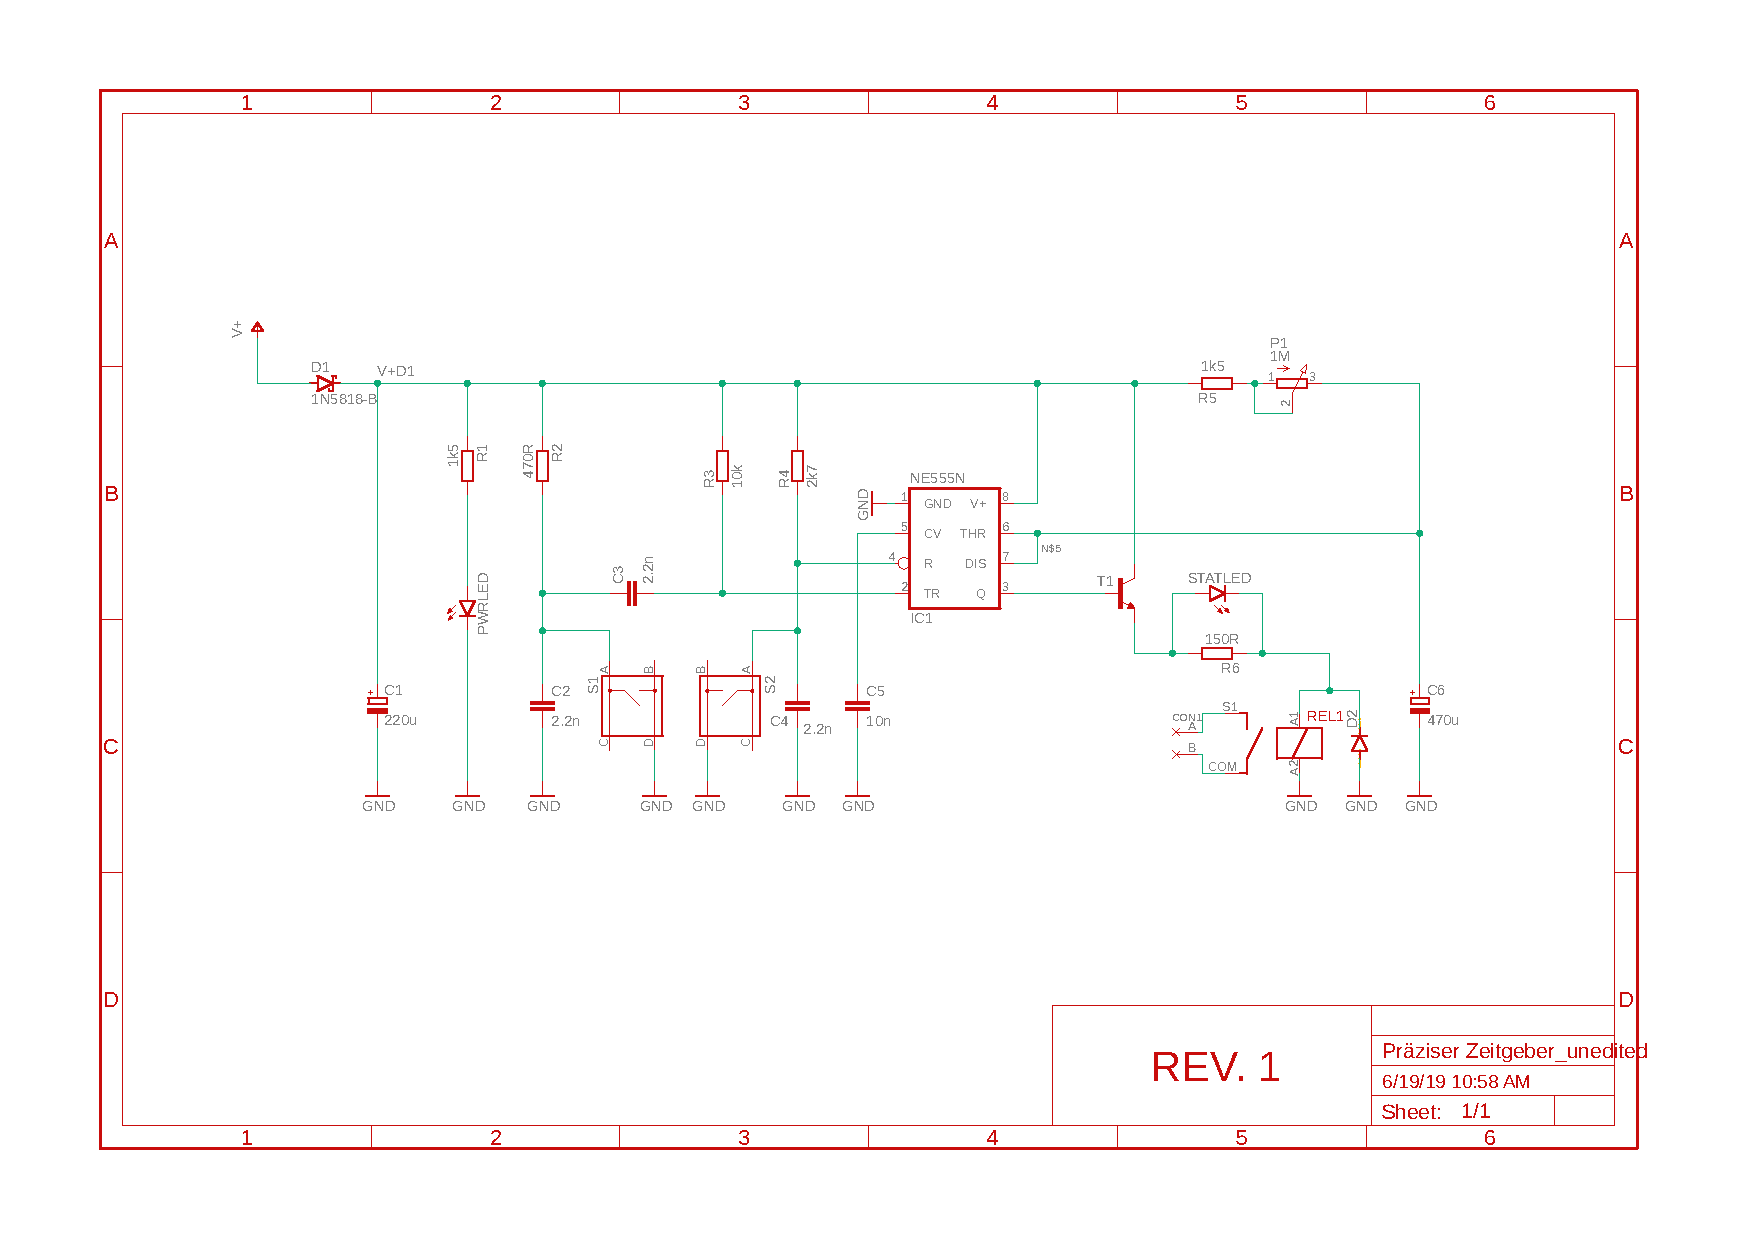
\includegraphics[page=1, scale=0.5]{graphics/PZ_unedited.pdf}
        \caption{Vorgegebener Schaltplan, unbearbeitet}
        \label{fig:1}
        \end{figure}

        \begin{figure}[H]
        \centering
        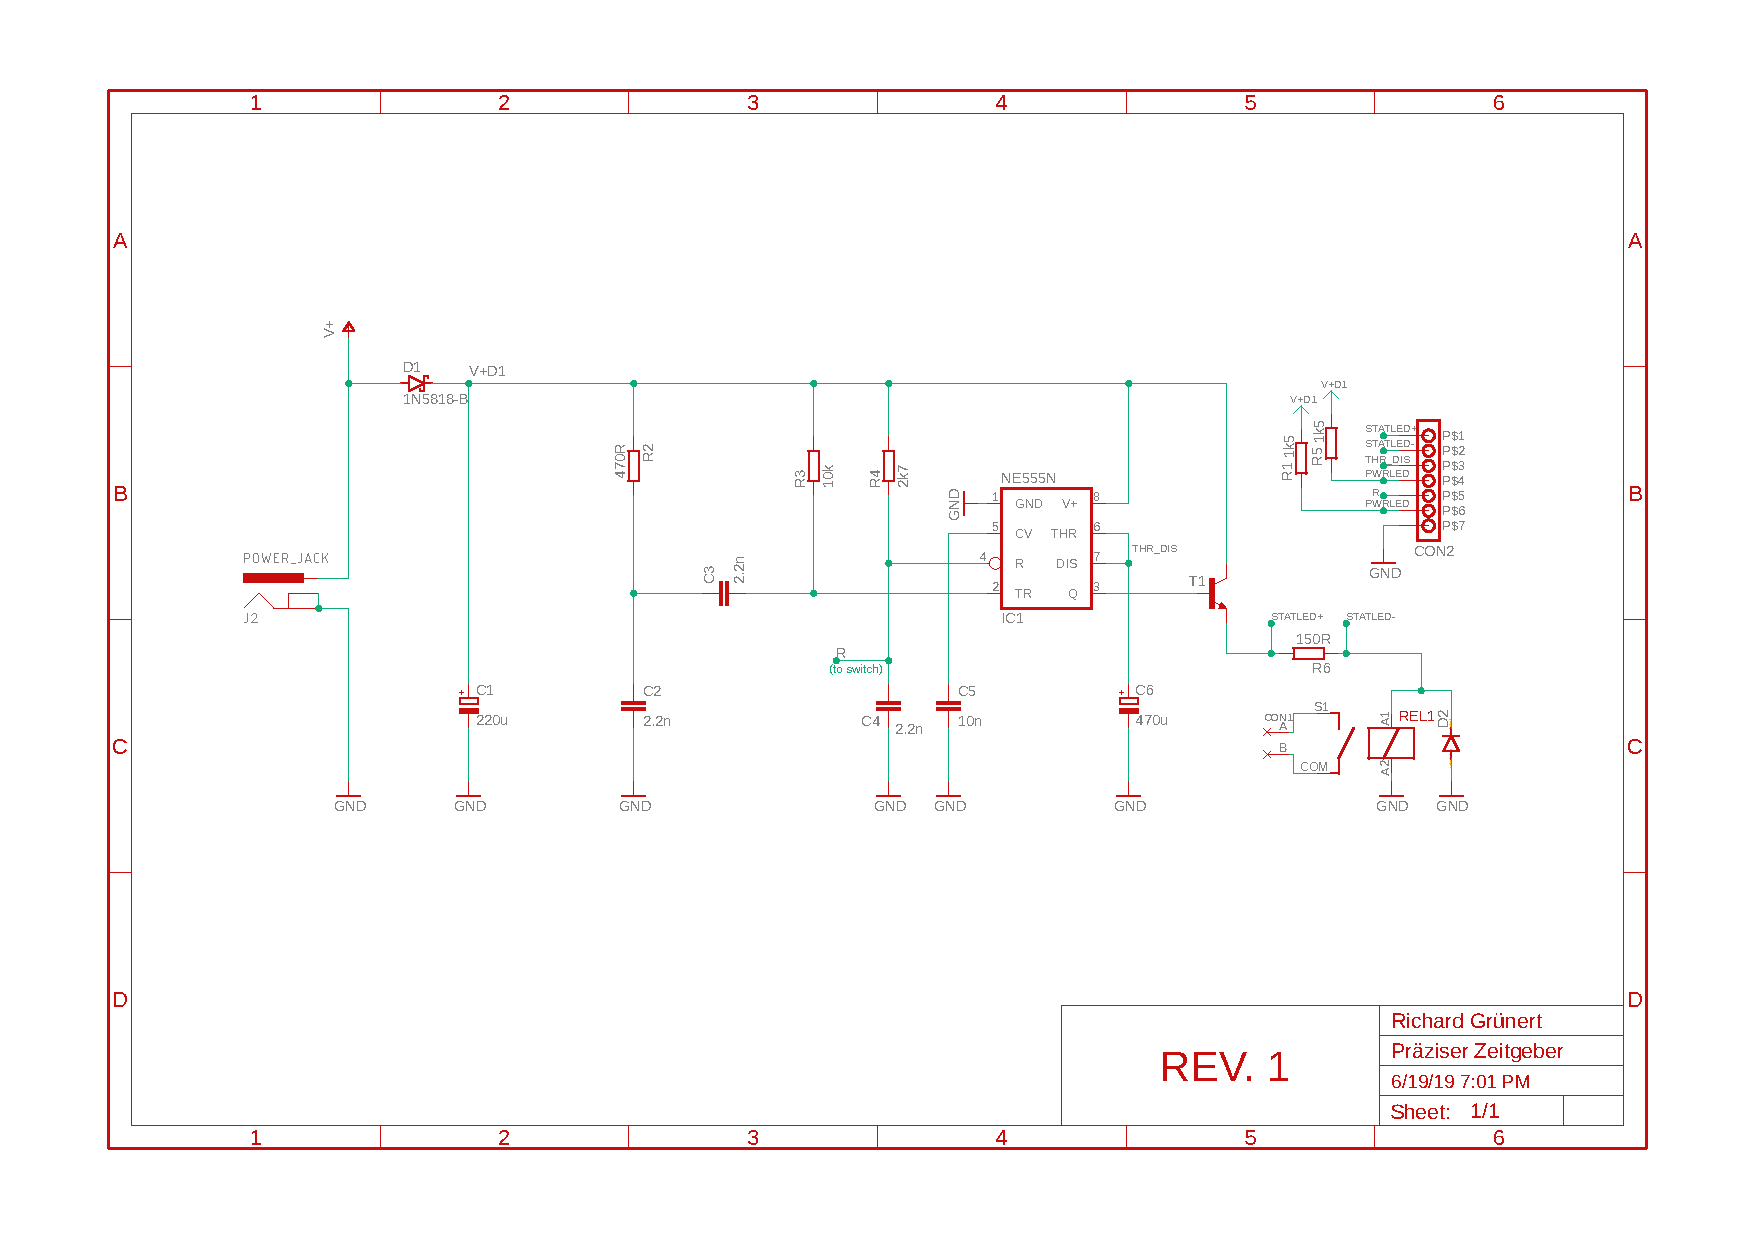
\includegraphics[page=1, scale=0.5]{graphics/PZ_schm}
        \caption{Vorgegebener Schaltplan, berarbeitet}
        \label{fig:2}
        \end{figure}





    \subsubsection{Bauteilliste}

    \begin{table}[H]
    \begin{center}
      \begin{tabular}{@{}cccc@{}}
        \toprule
        Art                            & Modell                           & Wert                        & Bezeichner          \\ \midrule
        \multirow{5}{*}{Widerstände}   & \multirow{5}{*}{Generisch, 0207} & $1.5 \,\ \si{\kilo\ohm}$    & $R1$, $R5$        \\
                                       &                                  & $470 \,\ \si{\ohm}$         & $R2$               \\
                                       &                                  & $10 \,\ \si{\kilo\ohm}$     & $R3$               \\
                                       &                                  & $2.7 \,\ \si{\kilo\ohm}$    & $R4$               \\
                                       &                                  & $150 \,\ \si{\ohm}$         & $R6$               \\ \midrule
        Potentiometer                  & Generisch                        & $1 \,\ \si{\mega\ohm}$      & $P_1$               \\ \midrule
        \multirow{4}{*}{Kondensatoren} & \multirow{2}{*}{Elektrolyt}      & $220 \,\ \si{\micro\farad}$ & $C_1$               \\
                                       &                                  & $470 \,\ \si{\micro\farad}$ & $C6$               \\
                                       & \multirow{2}{*}{Keramik}         & $2.2 \,\ \si{\nano\farad}$  & $C2$, $C3$, $C4$ \\
                                       &                                  & $10 \,\ \si{\nano\farad}$   & $C5$               \\ \midrule
        Transistor                     & BC547 oder BC237                 & –                           & $T2$               \\ \midrule
        \multirow{2}{*}{Dioden}        & 1N5818                           & –                           & $D1$               \\
                                       & 1N4148                           & –                           & $D2$               \\ \midrule
        \multirow{2}{*}{Leuchtdioden}  & 5mm, gelb                        & –                           & $LED1$              \\
                                       & 5mm, rot                         & –                           & $LED2$              \\ \midrule
        Schaltkreis                    & NE555                            & –                           & $IC1$              \\ \midrule
        IC-Sockel                  & DIL 8              & –                           & –              \\ \midrule
        Relais                         & BV2091                           & –                           & $REL1$             \\ \midrule
        Taster                         & Generisch, 6mm                   & –                           & $S1$, $S2$        \\ \midrule
        JST Steckverbinder             & JST-XHJST\_XH 7-Pin              & –                           & $CON2$              \\ \midrule
        Hohlstecker                    & 5,5 mm x 2,1 mm                  & –                           & $J2$                \\ \midrule
        Schraubklemme                  & JIEMIN JM2EDGV-R508              & –                           & $CON1$              \\ \bottomrule
      \end{tabular}
    \end{center}
    \caption{Bauteilliste}
    \end{table}

    \begin{figure}[H]
    \centering
    \begin{minipage}{.5\textwidth}
      \centering
      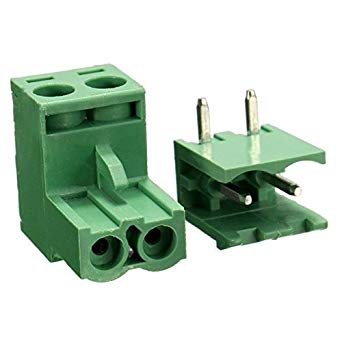
\includegraphics[width=.4\linewidth]{graphics/jiemin.jpg}
      \caption[Caption for LOF]{Klemme \emph{CON1}}
      \label{fig:3}
    \end{minipage}%
    \begin{minipage}{.5\textwidth}
      \centering
      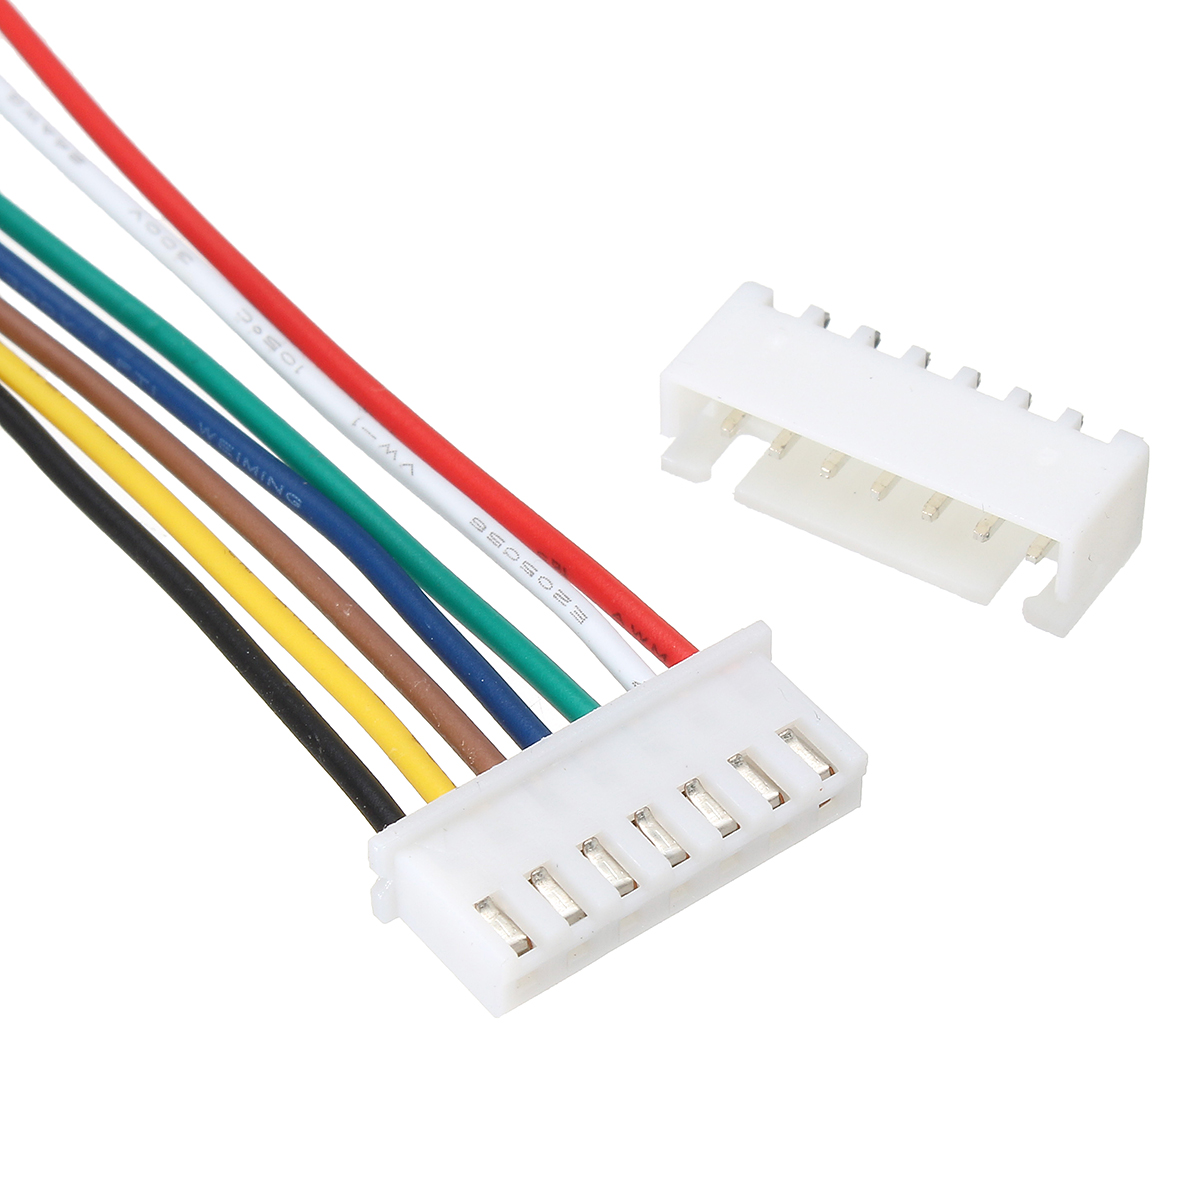
\includegraphics[width=.4\linewidth]{graphics/JST.png}
      \captionof{figure}{Verbindung \emph{CON2}}
      \label{fig:4}
    \end{minipage}
    \end{figure}

    %%%%%%%%%%%%%%%%%%%%%%%
    \subsubsection{Leiterplattenlayout}

        \begin{figure}[h]
        \begin{center}
          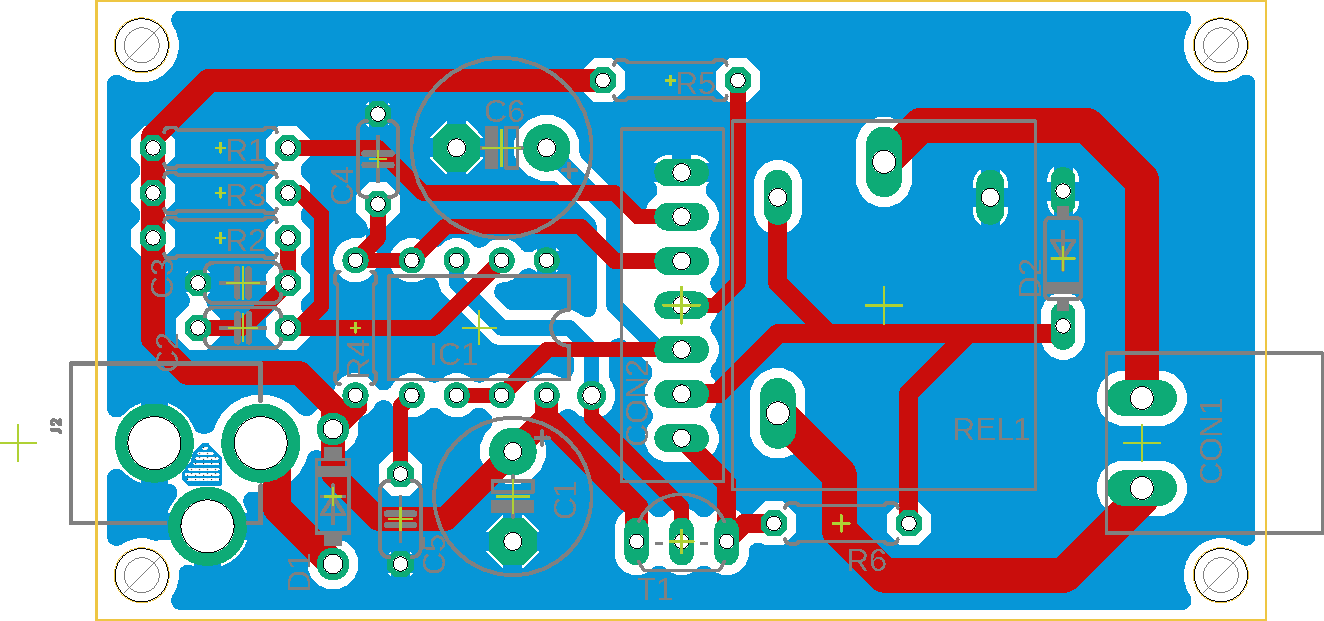
\includegraphics[page=1, scale=0.5]{graphics/layout.pdf}
          \caption{Layout der Schaltung}
          \label{fig:layout}
        \end{center}
        \end{figure}

        Die Leiterplatte wurde mithilfe des EDA Programms \textsc{Autodesk EAGLE} konstruiert.   Zur Konstruktion war es notwendig, neue Bibliotheken für das Relais, den JST-Header und die Klemmverbindung zu erstellen. Hierzu wurden die Daten der entsprechenden Datenblätter verwendet. Die Hohlbuchse $J2$ stammt aus der \textsc{SparkFun-Connectors} Bibliothek. Alle weiteren Bauteilmodelle wurden den Standard-EAGLE-Bibliotheken entnommen.\\

        Es wurde zuerst eine grobe Anordnung der größten Elemente (auf einer vorerst nicht festgelegten Fläche), wie den Verbindern, dem Relais und dem zentralen 555 Timer, sowie die Platzierung der Platinenbohrungen vorgenommen. Außerdem wurde der Kondensator $C1$ so nahe wie möglich an den Versorgungspins des Timers platziert, um mögliche Spannungseinbrüche bei dessen Schaltvorgängen auszugleichen. Bei der Positionierung der Klemme $CON1$ sowie der Hohlbuchse $J2$ und der Bohrungen wurde hier bereits auf die Verträglichkeit mit dem zukünfigten Gehäuse geachtet. Die verbleibenden Bauteile wurden ihrer Funktion und Position im Schaltplan entsprechend platziert. \\


        Die generelle Leiterbahnbreite für Verbindungen zwischen Komponenten beträgt 32 mil ($\approx 0.81\,\ \si{\milli\meter}$). Für die Versorgungsspannung wurde eine Breite von 50 mil ($\approx 1.27\,\ \si{\milli\meter}$), für den Relaisschalter 75 mil ($\approx 1.91\,\ \si{\milli\meter}$) gewählt, um die höheren Ströme (bis zu $3 \,\ \si{\ampere}$ durch das Relais) problemlos führen zu können. Zum Schluss wurde noch eine Massefläche auf der Bottom-Layer hinzugefügt, um den Fertigunsprozess zu beschleunigen.\\

        Nach der Umsetzung der Schaltung ist aufgefallen, dass der Schalter $S1$, der zum Auslösen des Zeitablaufes zuständig ist, übersehen wurde.\\

        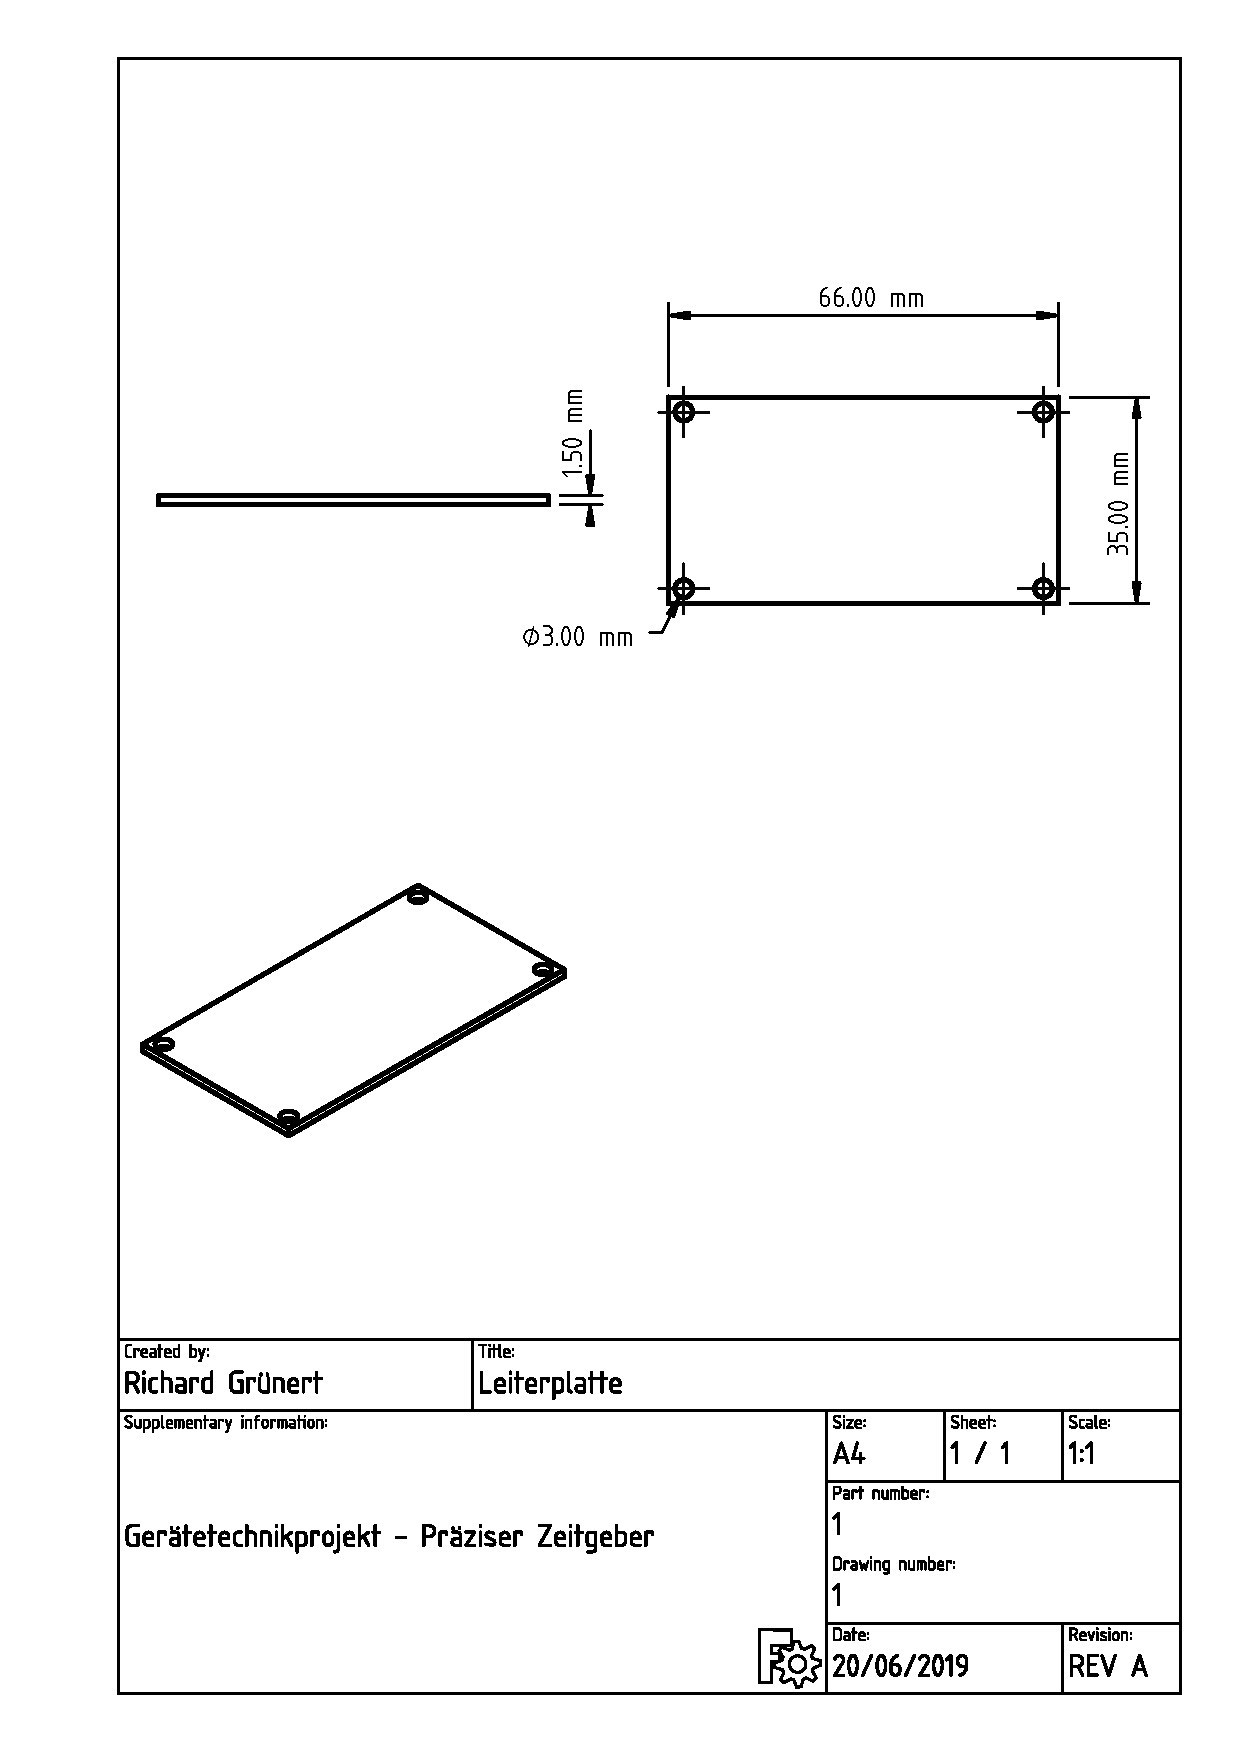
\includepdf{techdraw_platine.pdf}

    %%%%%%%%%%%%%%%%%%%%%%%
    \subsubsection{Gehäuse}
      Das für die Schaltung vorgesehene Gehäuse wurde mithilfe eines 3D-Druckers (FDM) umgesetzt. Konzeptionell besteht es aus zwei Bestandteilen:
      \begin{itemize}
        \item Unterhälfte \small mit Leiterplatte
        \item Oberhälfte \small mit Öffnungen für Potentiometer, LEDs und Taster
      \end{itemize}

      Der Entwurf dieser Teile wurde mit dem Programm \textsc{OpenSCAD} durchgeführt. \textsc{OpenSCAD} ist ein CAD Programm, in dem ein 3D-Modell durch Programmierung beschrieben wird. Diese Herangehensweise ermöglicht ein vollständig parametrisches Design, welches durch einfache Manipulation von Variablen eine schnelle Möglichkeit zur Erstellung von Prototypen und der Fehlerbehebung bietet. \\

      Besondere Herausforderung beim Entwurf des Gehäuses war die Umsetzung der Oberhälfte unter dem Aspekt der Kompaktheit. Das Relais hat hier als höchste Komponente die grundsätzliche Höhe des Gehäuses vorgegeben. Außerdem musste darauf geachtet werden, die Bauteile, die am Gehäuse befestigt wurden, im Design präzise zu platzieren, damit sie nicht mit anderen Bauteilen innerhalb des Gehäuses kollidieren. \\

      Das Gehäuse wurde in transparentem und rotem Polylactid (PLA) bei einer Layer Height von $0.12 \,\ \si{\milli\meter}$ und einer Infill Dichte von $13 \,\ \%$ gedruckt und schließlich leicht mit einer Feile bearbeitet.\\

      Die virtuellen Modelle sind in Abb. \ref{fig:3d1} und Abb. \ref{fig:3d2}, die gedruckten Gehäuseteile in Abb. \ref{fig:gedruckt1} und Abb. \ref{fig:gedruckt2} zu sehen. Der entsprechende Programmcode befindet sich im Anhang.

      \begin{center}
        \begin{figure}[H]
        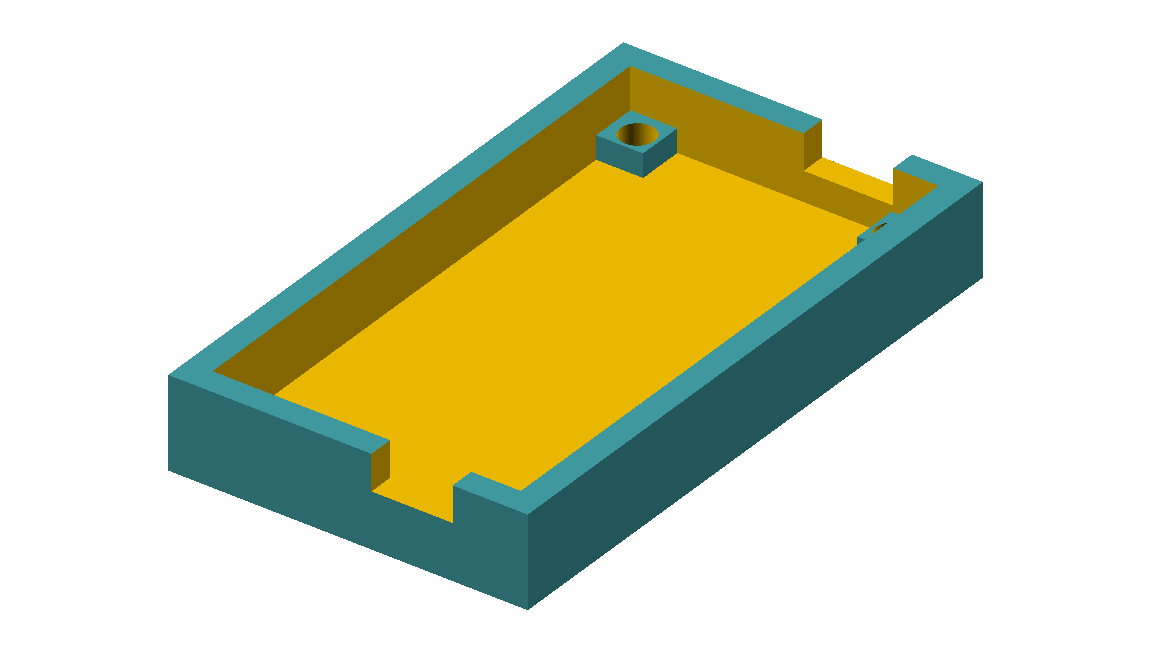
\includegraphics[page=1, scale=0.5]{graphics/Gehaeuse_bottom.png}
        \caption{Unterhälfte des Gehäuses}
        \label{fig:3d1}
        \end{figure}
      \end{center}

      \begin{center}
        \begin{figure}[H]
        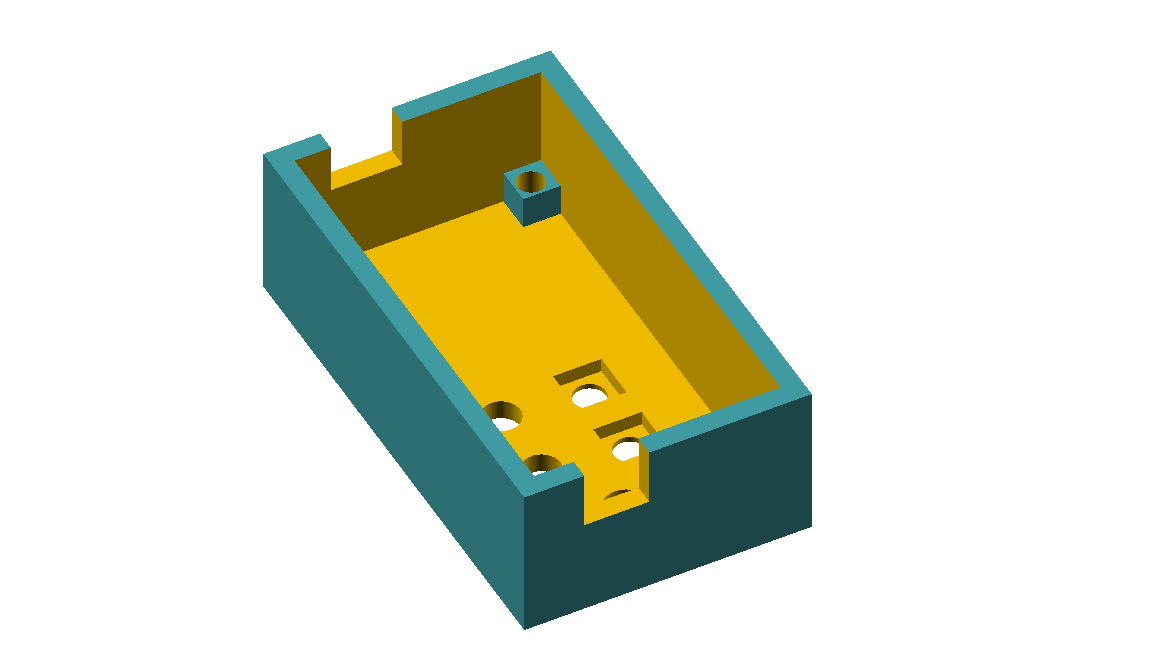
\includegraphics[page=1, scale=0.5]{graphics/Gehaeuse_top_test.png}
        \caption{Oberhälfte des Gehäuses}
        \label{fig:3d2}
        \end{figure}
      \end{center}


      \begin{figure}[h!]
      \centering
        \begin{minipage}{.5\textwidth}
          \centering
          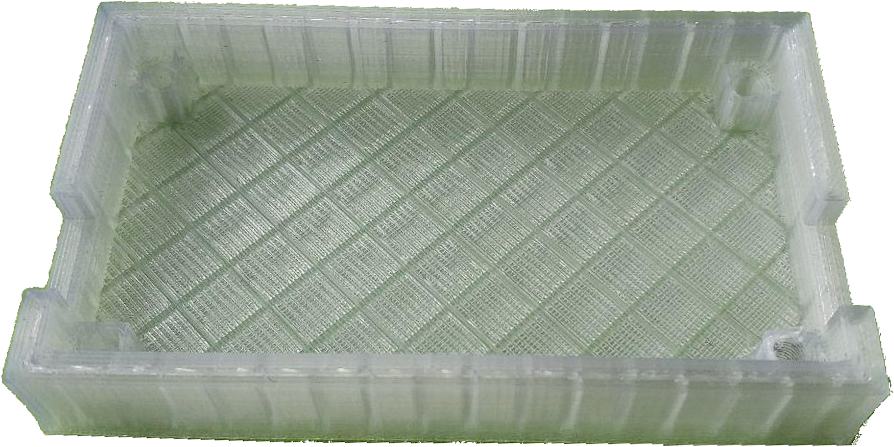
\includegraphics[width=.9\linewidth]{graphics/gehaeuse_gedruckt_unten.jpg}
          \captionof{figure}{Gedruckte Unterhälfte}
          \label{fig:gedruckt1}
        \end{minipage}%
        \begin{minipage}{.5\textwidth}
          \centering
          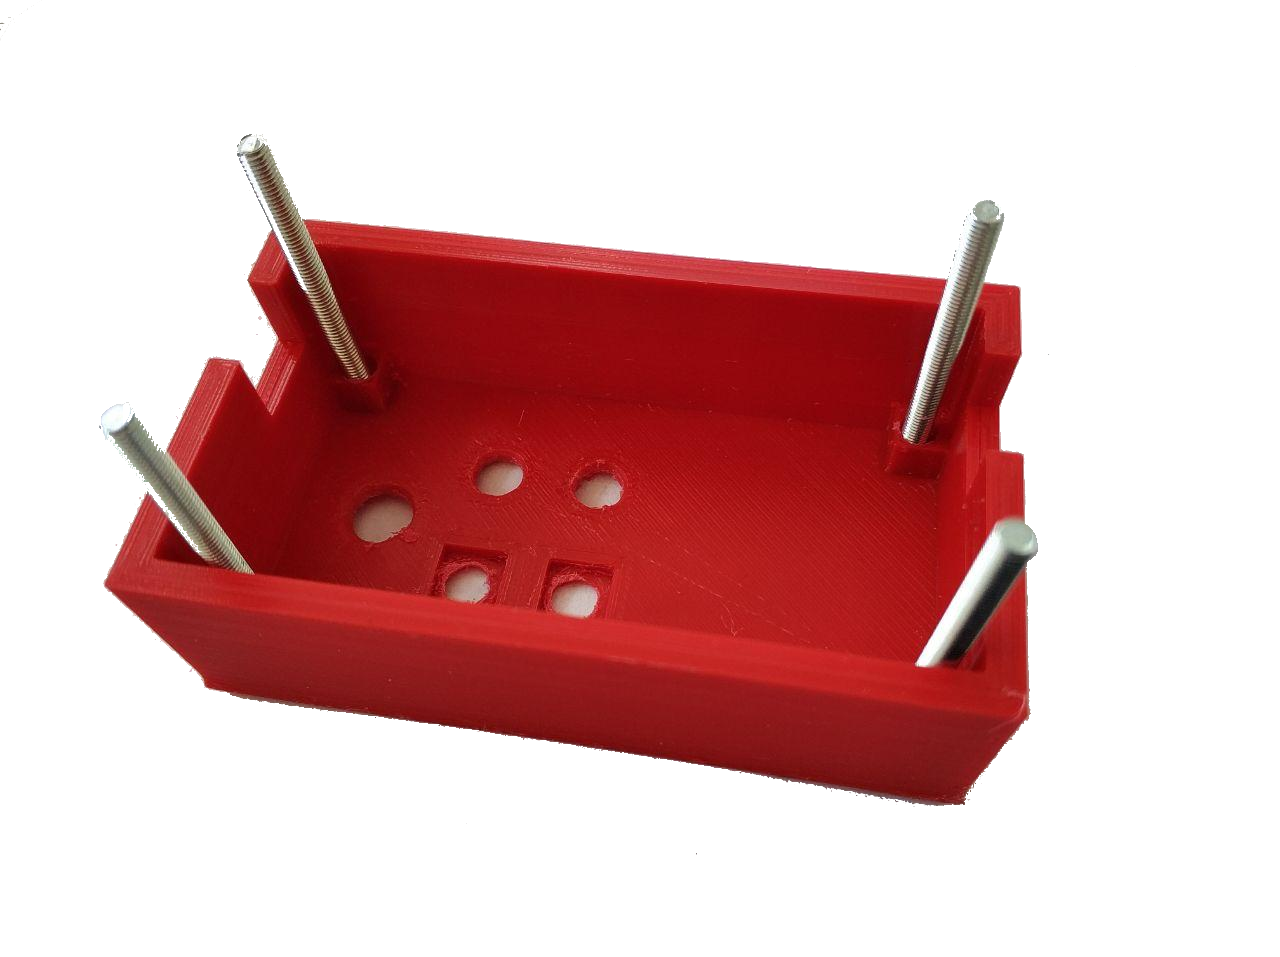
\includegraphics[width=.9\linewidth]{graphics/gehaeuse_gedruckt_oben.png}
          \captionof{figure}{Gedruckte Oberhälfte (mit Schrauben)}
          \label{fig:gedruckt2}
        \end{minipage}
      \end{figure}



  %%%%%%%%%%%%%%%%%%%%%%%
  \subsection{Fertigung}

    \subsubsection{Details}

    Die Leiterplatte wurde in der \emph{Zentralwerkstatt der Hochschule Wismar} gefertigt. Sie besteht aus Epoxid; die Leiterbahnen wurden verzinnt. Lötstopplack ist jedoch nicht vorhanden. Bei der Bestückung wurde bemerkt, dass der Footprint des Relais' gespiegelt war, was durch Korrektur des Layouts und Neuanfertigung der Platine behoben werden konnte. Zudem wurde im ersten Entwurf eine inkorrekte EAGLE Bibliothek mit falschen Bohrungen für die Steckverbindung der Spannungsversorgung verwendet, was jedoch durch die Verwendung der Steckverbindung aus der \textsc{SparkFun-Connectors-Bibliothek} ebenfalls leicht behoben werden konnte (Abb. \ref{fig:fehler1}, Abb. \ref{fig:korr1}).\\

    \begin{figure}[H]
    \centering
      \begin{minipage}{.5\textwidth}
        \centering
        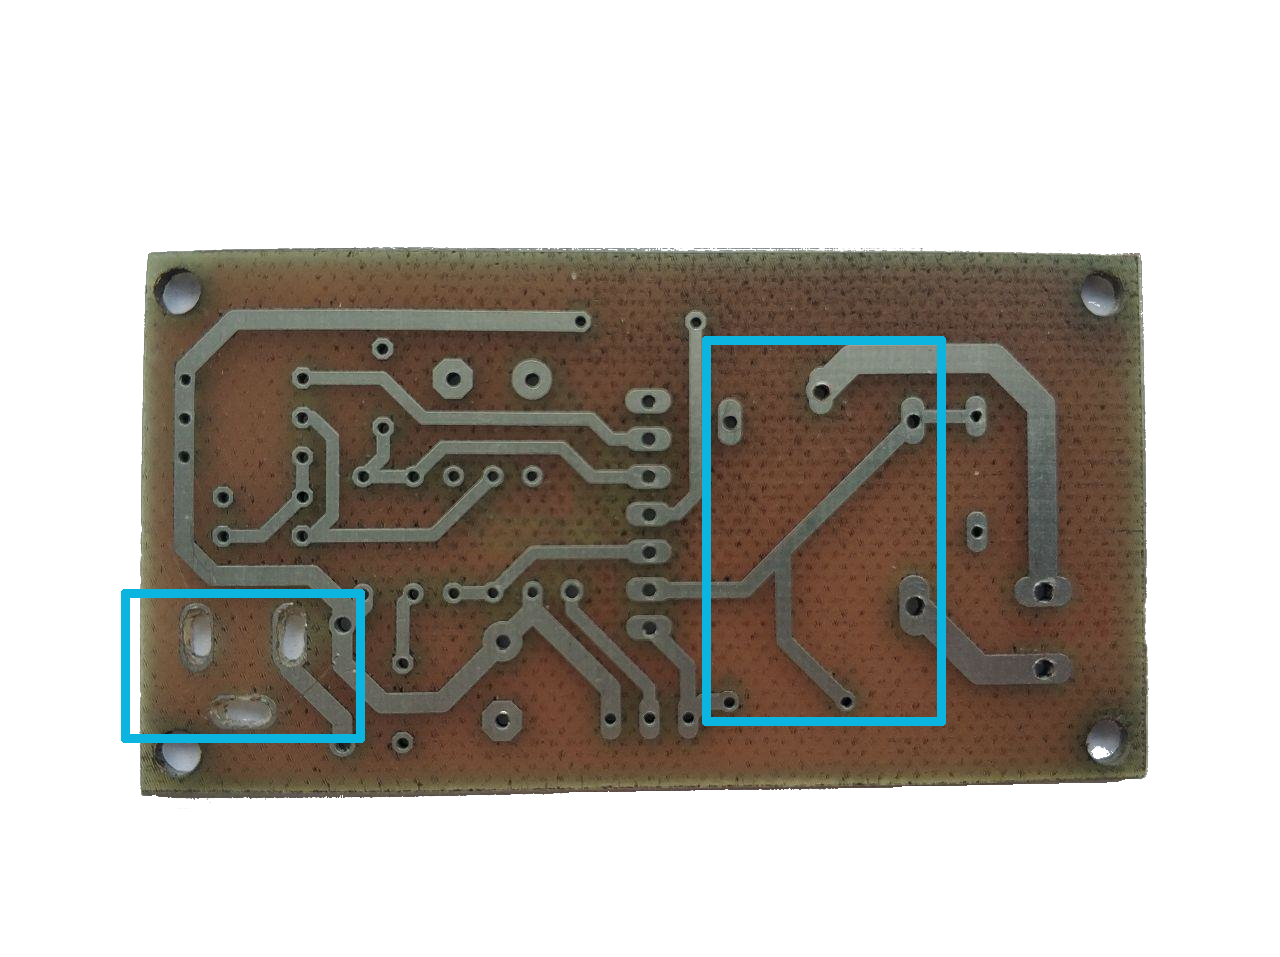
\includegraphics[width=.9\linewidth]{graphics/f2.png}
        \captionof{figure}{Fehlerhafte Leiterplatte}
        \label{fig:fehler1}
      \end{minipage}%
      \begin{minipage}{.5\textwidth}
        \centering
        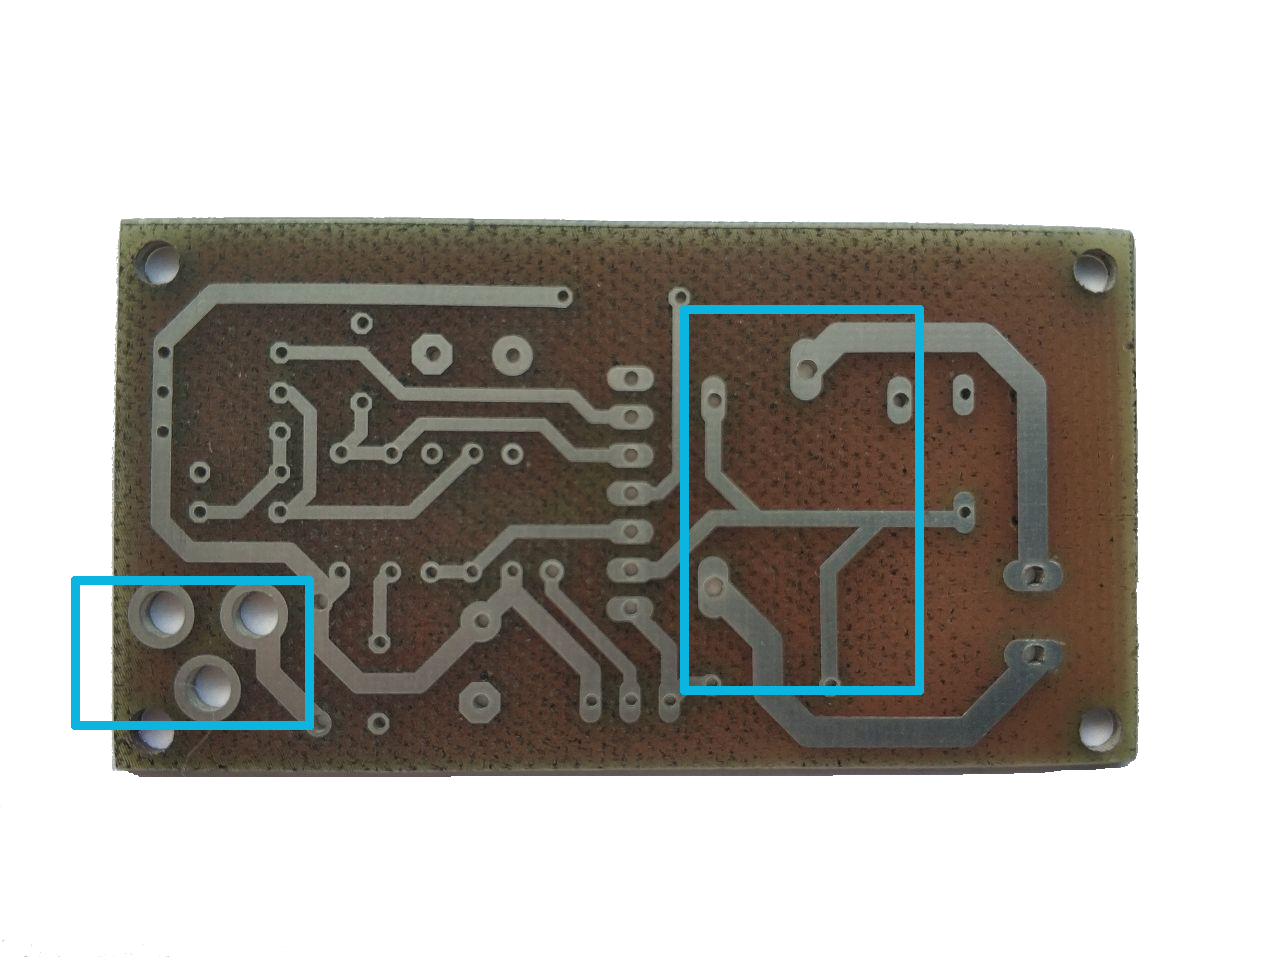
\includegraphics[width=.9\linewidth]{graphics/k3.png}
        \captionof{figure}{Korrigierte Leiterplatte}
        \label{fig:korr1}
      \end{minipage}
    \end{figure}


    \subsubsection{Bestückung}
    Bei der Bestückung der Leiterplatte wurden zuerst die kleinsten Bauteile, wie Widerstände und Keramikkondensatoren, danach die größeren, wie Steckverbindungen, und das Relais verlötet. Vor dem Verlöten der jeweiligen Bauteile wurde deren Wert gemessen und keine beeinträchtigenden Abweichungen festgestellt. Weitere Tests (z.B. Durchlassprüfungen) nach dem Löten zeigten eine fehlerfreie Bestückung. Zusätzlich zur Bestückung musste der Stecker für die JST-Verbindung zusammengesetzt werden (Abb. \ref{fig:jstloet}). Die dabei verwendeten Jumper-Kabel sind für die relativ geringen Ströme geeignet dimensioniert. Am anderen Ende wurden die Bauteile \emph{P1, STATLED, PWRLED, S1 und S2} befestigt, wobei der Schaft des Potentiometers noch eingekürzt wurde, um in einen Drehknopf zu passen. Danach wurden sie an Gehäuseoberseite in den vorgesehenen Öffnungen mit Flüssigkleber befestigt (Abb. \ref{fig:klebi}). Das zusammengesetzte Gehäuse wurde schließlich mit M3-Schrauben und -Muttern geschlossen und ist in Abb. \ref{fig:gehaeuse} und Abb. \ref{fig:erklaer} zu sehen.\\

    Der im Layout fehlende Schalter $S1$ wurde durch ein Kabel am Widerstand $R2$ ersetzt, welches das Funktionsproblem behebt, jedoch das Ziel der Modularität erschwert. Als Masseverbindung für den Schalter wurde die Masse der JST-Verbindung verwendet, da diese bereits am oberen Gehäuse verfügbar war.\\

    Die vollständig bestückte Platine ist in Abb. \ref{fig:bestueckt1} und Abb. \ref{fig:bestueckt2} zu sehen.

    \begin{figure}[H]
    \begin{center}
    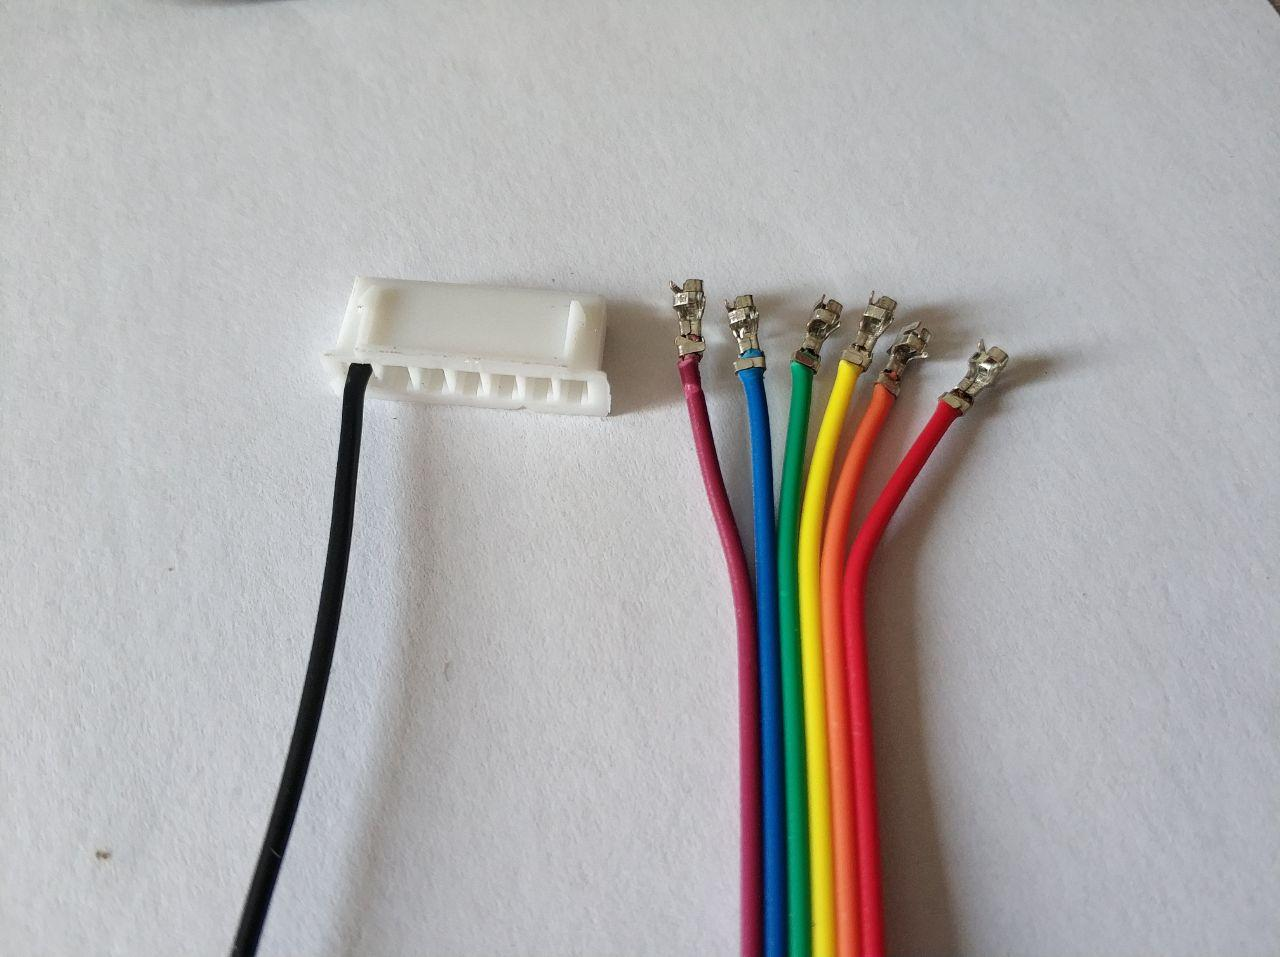
\includegraphics[page=1, width=0.5\linewidth]{graphics/jstloet.jpg}
    \caption{Zusammensetzung des Steckverbinders}
    \label{fig:jstloet}
    \end{center}
    \end{figure}


    \begin{figure}[h!]
    \centering
      \begin{minipage}{.5\textwidth}
        \centering
        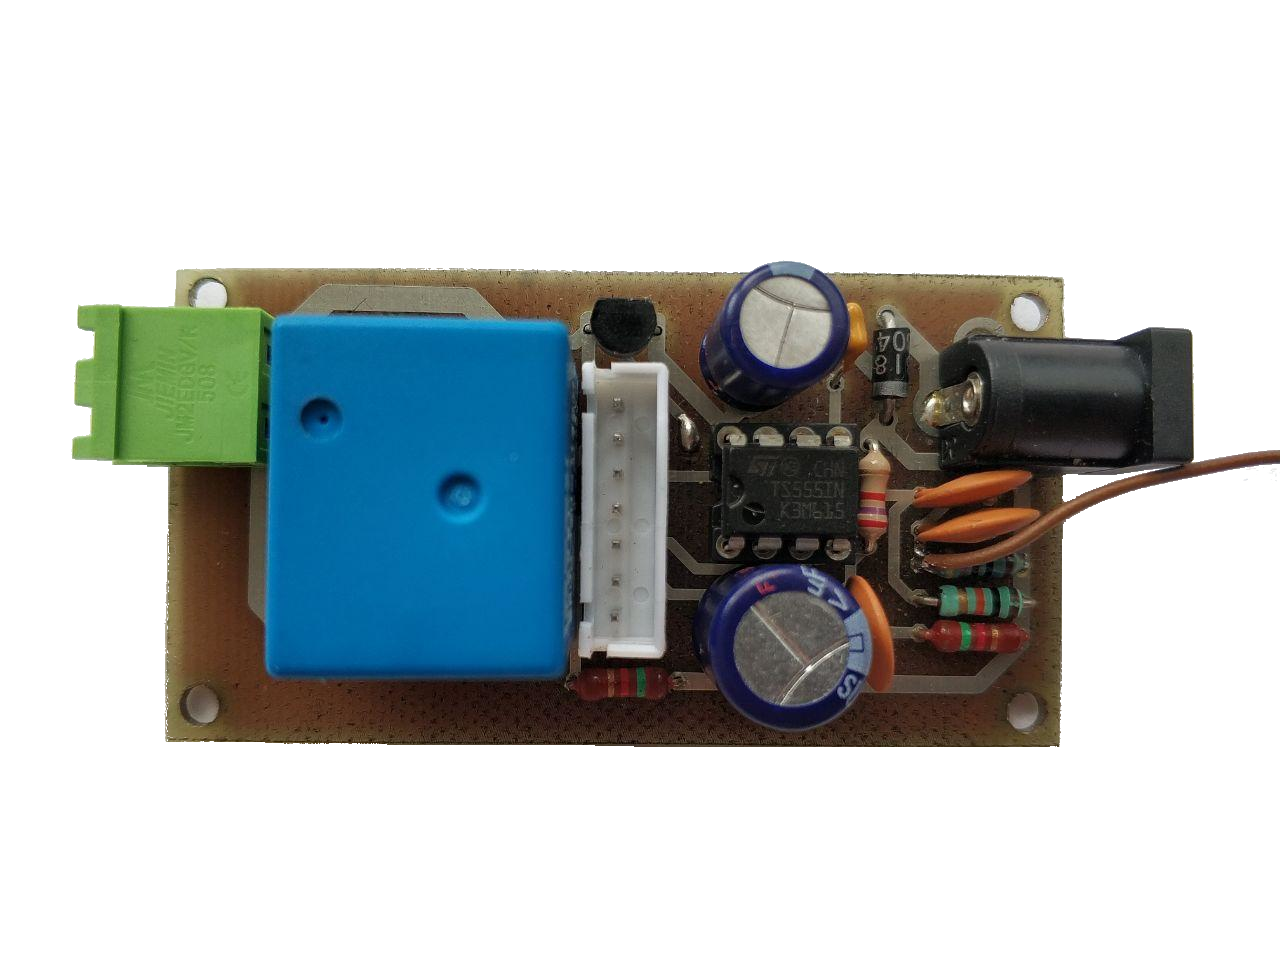
\includegraphics[width=.9\linewidth]{graphics/bestueckt_oben.png}
        \captionof{figure}{Leiterplatte bestückt, oben}
        \label{fig:bestueckt1}
      \end{minipage}%
      \begin{minipage}{.5\textwidth}
        \centering
        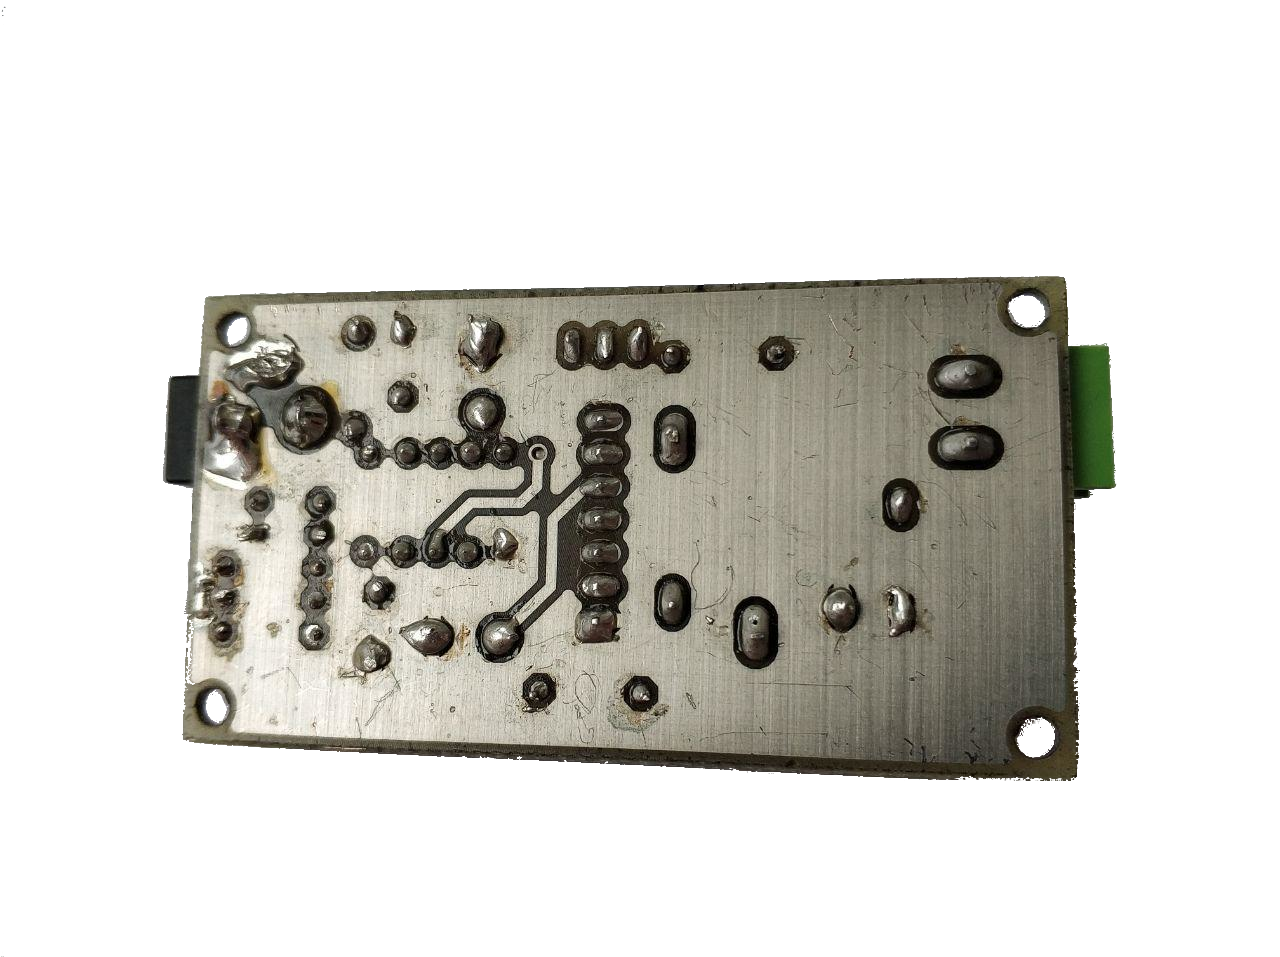
\includegraphics[width=.9\linewidth]{graphics/bestueckt_unten.png}
        \captionof{figure}{Leiterplatte bestückt, unten}
        \label{fig:bestueckt2}
      \end{minipage}
    \end{figure}

    \begin{figure}[H]
      \begin{center}
      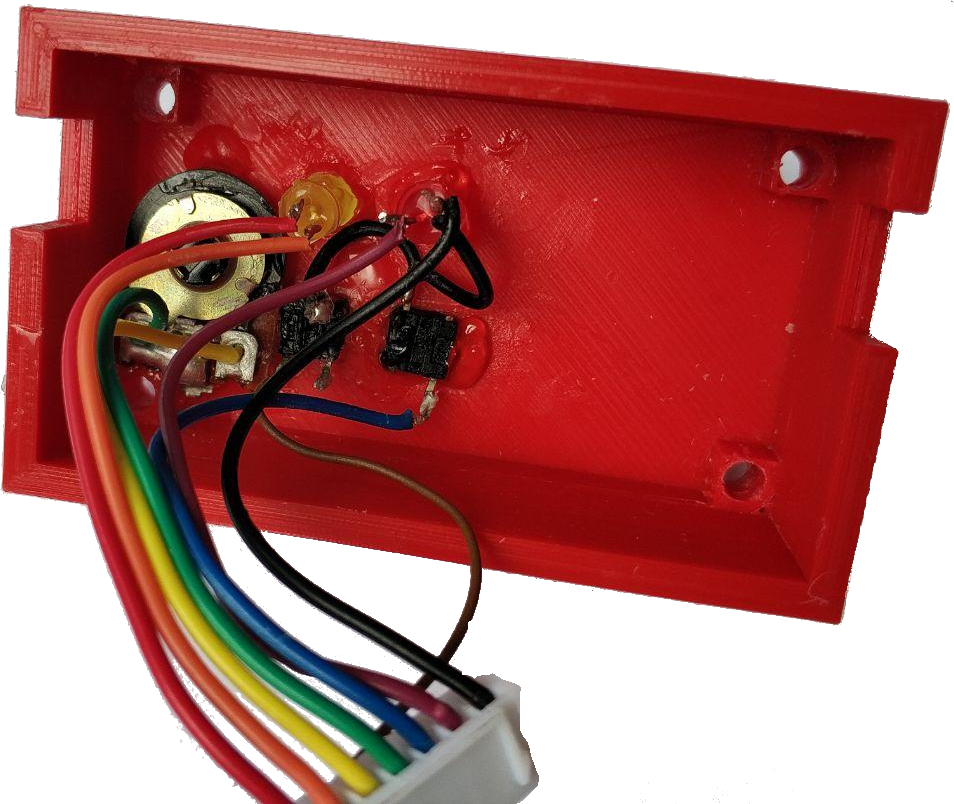
\includegraphics[page=1, width=0.5\linewidth]{graphics/klebi.png}
      \caption{Geklebte Bauteile am Gehäuse}
      \label{fig:klebi}
      \end{center}
    \end{figure}

    \begin{figure}[H]
      \begin{center}
      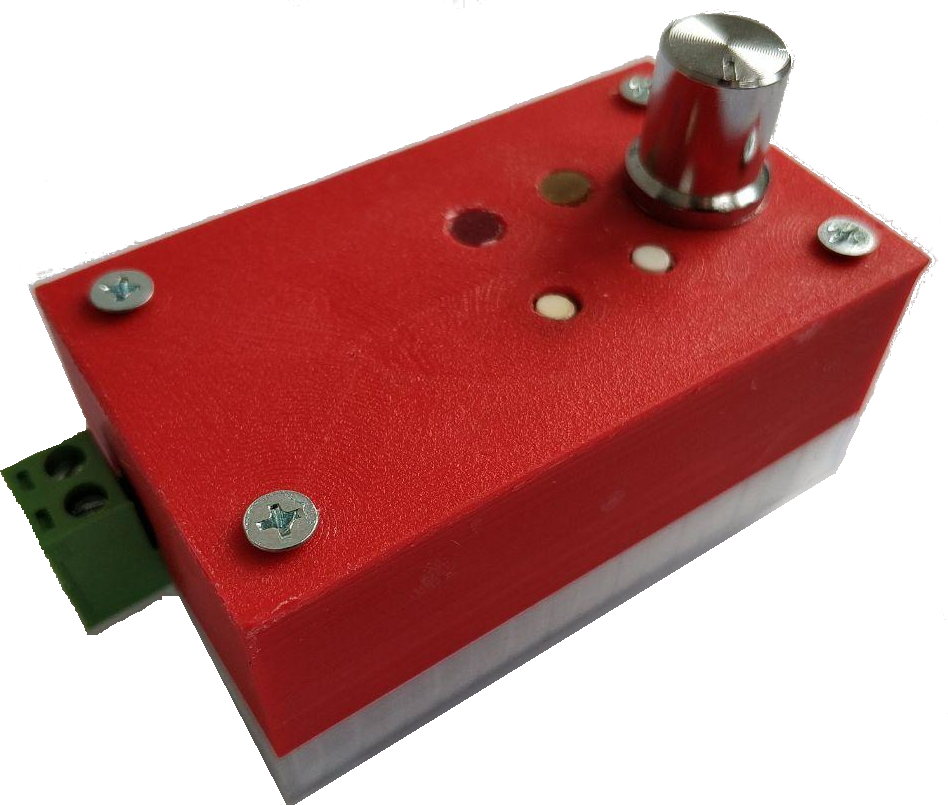
\includegraphics[page=1, width=0.5\linewidth]{graphics/gehaeuse.png}
      \caption{Vollständiges Gehäuse}
      \label{fig:gehaeuse}
      \end{center}
    \end{figure}

    \begin{figure}[H]
      \begin{center}
      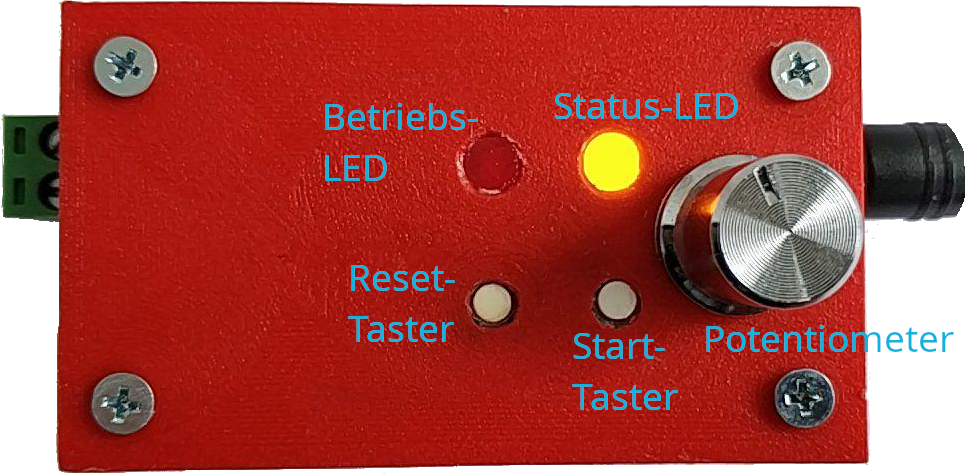
\includegraphics[page=1, width=0.5\linewidth]{graphics/gehaeuse_bezeichnung.png}
      \caption{Anordnung der Gehäusebauteile}
      \label{fig:erklaer}
      \end{center}
    \end{figure}

  %%%%%%%%%%%%%%%%%%%%%%%
  \subsection{Funktionsnachweis}
    Zur Überprüfung der Funktion wurde mit einem LCR-Meter der Durchlass an den Klemmen $CON1$ bei mehreren Potentiometerstellungen gemessen, während die Schaltung durch ein einfaches $12 \,\ \si{\volt}$ Netzteil betrieben wurde. Dabei ließen sich keine Fehler feststellen (Abb. \ref{fig:messi1}, Abb. \ref{fig:messi2}).
    Mithilfe des Potentiometers lassen sich Zeitintervalle von etwa $1 \,\  \si{\second}$ bis $10 \,\  \si{\minute}$ einstellen.

    \begin{figure}[h!]
    \centering
      \begin{minipage}{.5\textwidth}
        \centering
        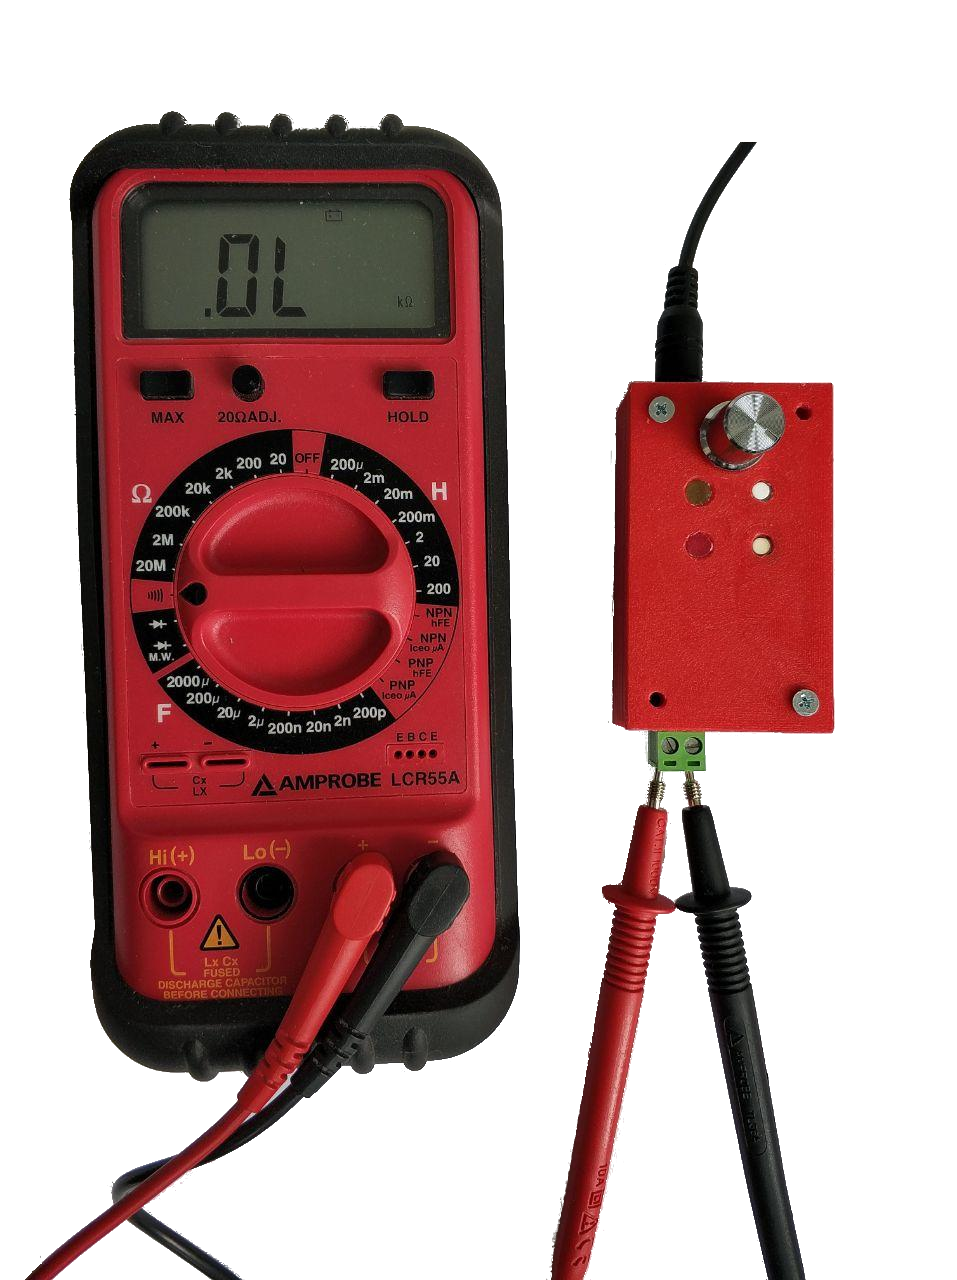
\includegraphics[width=.9\linewidth]{graphics/messi1.png}
        \captionof{figure}{\small Messung bei inaktivem Relais}
        \label{fig:messi1}
      \end{minipage}%
      \begin{minipage}{.5\textwidth}
        \centering
        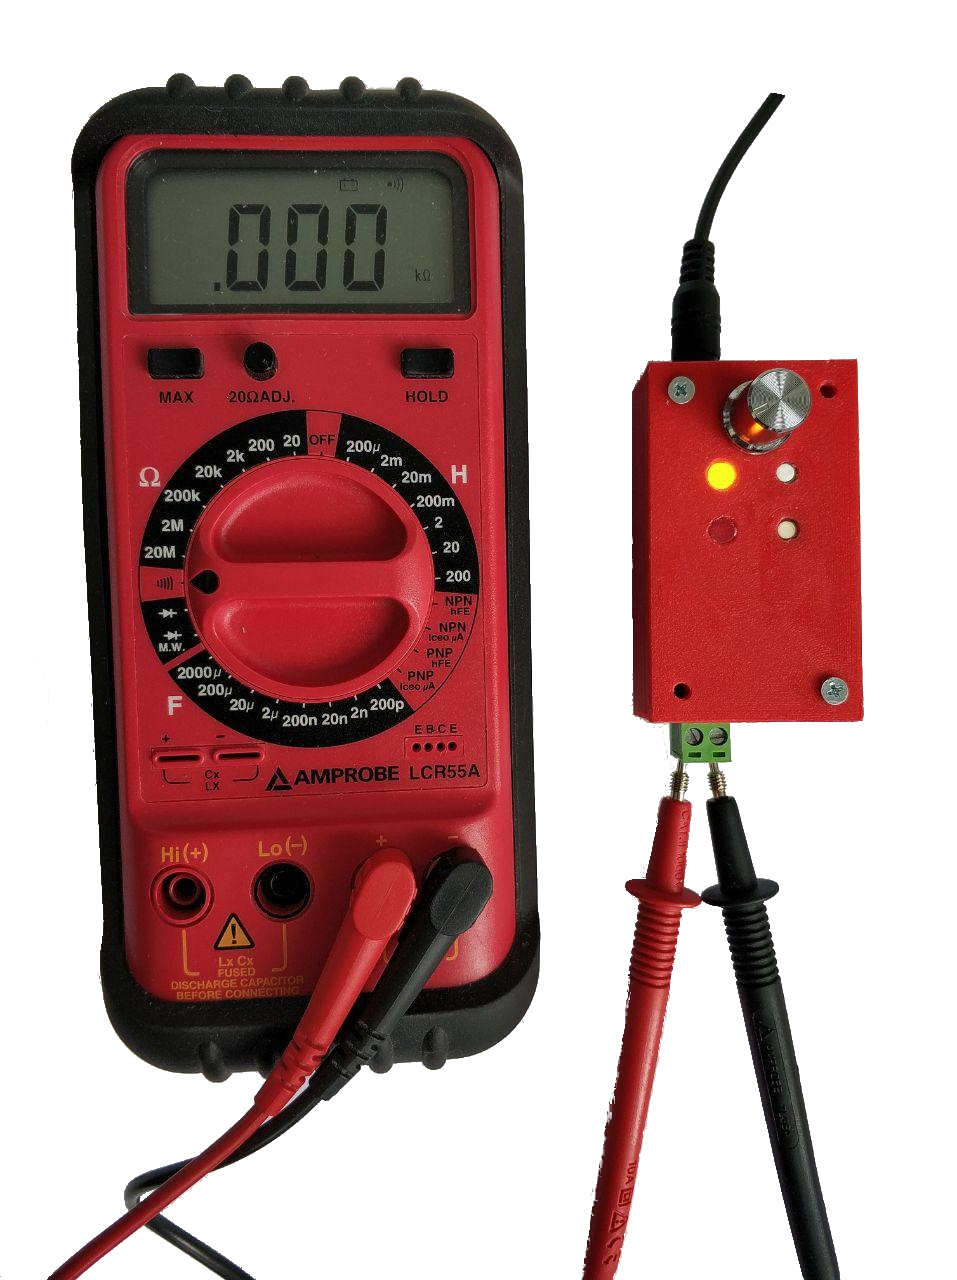
\includegraphics[width=.9\linewidth]{graphics/messi2.png}
        \captionof{figure}{\small Messung bei aktivem Relais}
        \label{fig:messi2}
      \end{minipage}
    \end{figure}

    Da es sich bei diesem Projekt um eine einfache Gleichstromschaltung handelt und daher keine hochfrequenten Schaltvorgänge stattfinden, ist eine EMV-Betrachtung an dieser Stelle nicht notwendig.

  \subsection{Leistung und thermische Betrachtung}
    Im Labor der Hochschule Wismar wurde mithilfe eines Labornetzteils und Multimeters die minimal benötigte Spannung zum Betrieb der Schaltung $U_{\text{min}} = 10.6 \,\ \si{\volt}$ ermittelt. Die allgemeine Betriebsspannung liegt bei $U = 12 \,\ \si{\volt}$. Der dabei fließende Strom ist vom Zustand der Schaltung abhängig:\\


      Bei ausgeschaltetem Relais: $$I_{\text{low}} = 14.1 \,\ \si{\milli\ampere}$$
      \indent Bei eingeschaltetem Relais: $$I_{\text{high}} = 28.2 \,\ \si{\milli\ampere} \approx 30 \,\ \si{\milli\ampere}$$


    Für den Worst-Case-Fall wird hier von einem Strom von $I = 50 \,\ \si{\milli\ampere}$ ausgegangen. Die maximale Leistungsaufnahme ist somit:

    $$P = 12 \si{\volt} \cdot 50 \si{\milli\ampere} = 600 \,\ \si{\milli\watt}$$\\

    Das Relais ist hierbei das leistungsintensivste Bauelement. Bei etwa $20 \,\ \si{\celsius}$ wurde ein Spulenwiderstand von $400 \,\ \si{\ohm}$ ermittelt. Rechnet man den Relaisstrom über die Stromdifferenz $I_{\text{high}}-I_{\text{low}}$ auf den Worst-Case-Fall hoch, erhält man:

    $$I_{\text{REL}_{\text{WC}}} = \frac{50\si{\milli\ampere}}{28.2\si{\milli\ampere}} \cdot (28.2 - 14.1)\si{\milli\ampere}= 25 \,\ \si{\milli\ampere}$$\\

    \noindent und somit eine Leistung von

    $$P_{\text{REL}_{\text{WC}}} = (25 \,\ \si{\milli\ampere})^2 \cdot 400 \si{\ohm} =  250 \,\ \si{\milli\watt}$$

    Aus dem Datenblatt des Relais lässt sich bei dieser Leistung eine Temperaturerhöhung der Relaisspule von etwa $15 \,\ \si{\celsius}$ aus deren Kennlinie ablesen, was jedoch innerhalb des empfohlenen Maximalwertes ($35 \,\ \si{\celsius}$) liegt, weshalb keine Kühlmaßnahmen benötigt wurden. Dies ist natürlich nur eine grobe Abschätzung, zeigt aber, dass selbst unter Annahme eines erhöhten \emph{Betriebsstromes} keine Gefahr der Überhitzung besteht.


  \subsection{Verbesserungsmöglichkeiten}
    Eine potentielle Verbesserung des Projekts ist die Platzeinsparung am äußeren Ende der Leiterplatte bei $CON1$ (Abb. \ref{fig:sparen}).
    Eine weitere ist der Entwurf einer separaten Platine zur Befestigung der Bauteile am Gehäuse (LED, Potentiometer, etc. ), die lediglich Routes zu einem JST-Verbinder führen würde. Dies wäre eine stabilere, modularere und bei Fertigung verlässlichere Bauweise gegenüber der Klebbefestigung, besonders, da der Schalter $S2$ in diesem Projekt am Gehäuse durch den Klebstoff funktionsunfähig wurde. Eine alternative Lösung hierfür ist, das Gehäusemodell so zu bearbeiten, dass es geeignete ``Slots'' für Bauteile bereitstellt, in welchen diese gehalten werden können. Weiterhin könnten zum Verschluss des Gehäuses Schrauben verwendet werden, welche auf dessen Höhe angepasst sind, um einen Überstand zu vermeiden.\\

    Der wichtigste Verbesserungsaspekt ist jedoch die Layoutanpassung zur Berücksichtigung des vergessenen Schalters $S1$. Dies benötigt eine Erweiterung des JST-Verbinders von 7 auf 8 Pins, sowie eine Route vom Widerstand $R2$ bzw. Kondensator $C3$ zu diesem Verbinder, was z.B. einfach über die Bottom-Layer realisiert werden könnte (Abb. \ref{fig:schalterkorrektur})).\\

    \begin{figure}[h]
    \begin{center}
      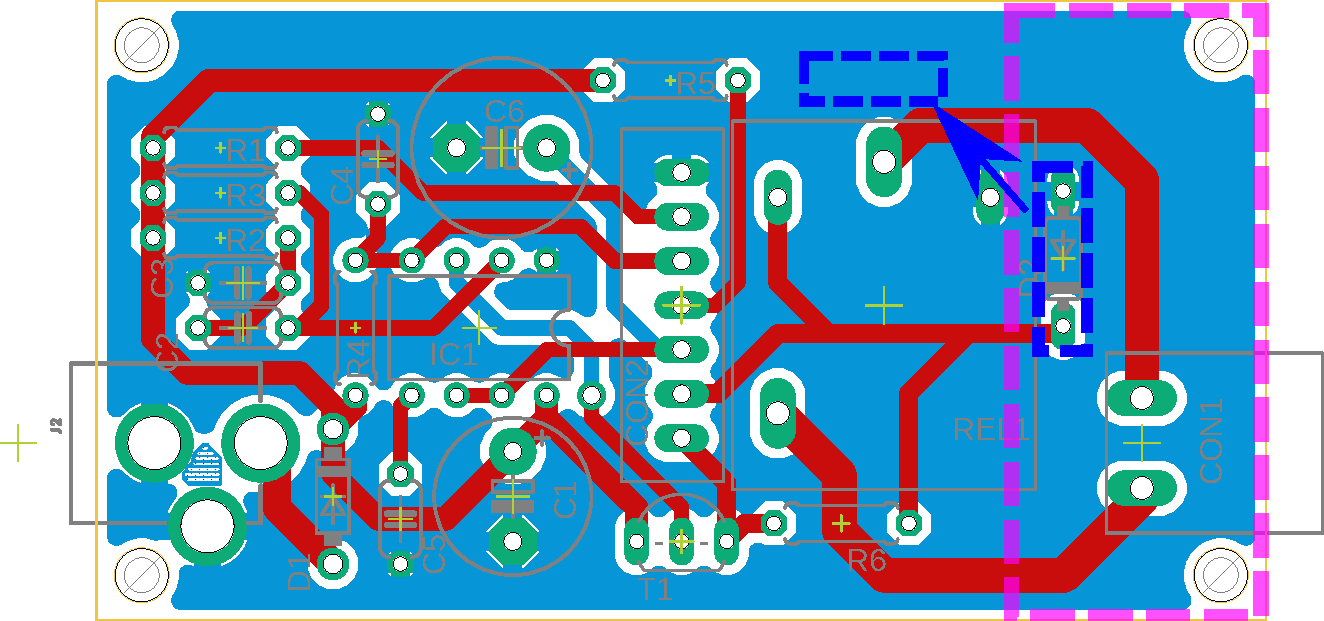
\includegraphics[page=1, scale=0.5]{graphics/sparen.pdf}
      \caption{Mögliche Platzoptimierung z.B. durch andere Plazierung der Diode $D2$}
      \label{fig:sparen}
    \end{center}
    \end{figure}

    \begin{figure}[h]
    \begin{center}
      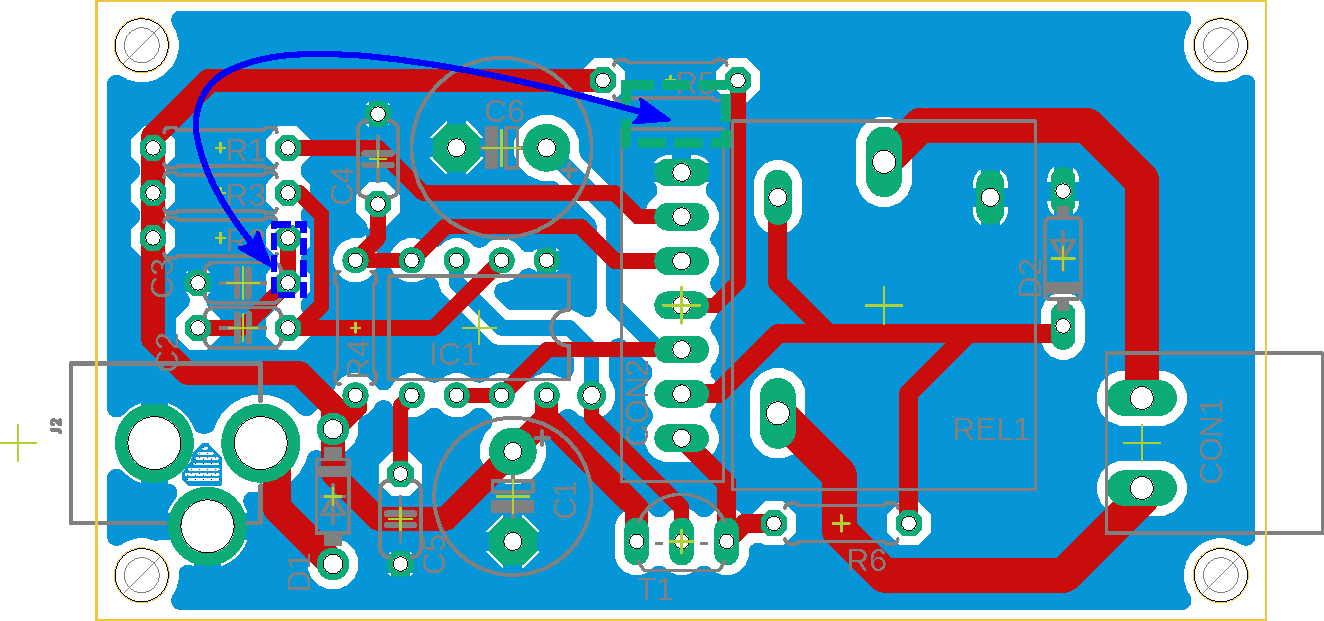
\includegraphics[page=1, scale=0.5]{graphics/schalterkorrektur.pdf}
      \caption{Mögliche Einführung des Schalters $S1$ }
      \label{fig:schalterkorrektur}
    \end{center}
    \end{figure}



\section{Zusammenfassung}
Das Projekt des Moduls \emph{Gerätetechnik} erwies sich persönlich als sehr erfolgreich. Ich habe Grundlagen des konstruktiven Entwicklungsprozesses von Leiterplatten, darunter u.a. die rechnergestützte Konstruktion, sowie technische Herangehensweisen an entsprechende Problemstellungen und Planung der Lösung dieser erfahren können. Gerade der Umgang mit Fehlern und die Problemlösung wurden (u.a. da Fehler in der Konstruktion auftraten) in diesem Zusammenhang umfangreich behandelt. Das Leiterplattenlayout ist aus meiner Sicht (unter Vernachlässigung des fehlenden Schalters $S1$) gut gelungen; es entstand ein funktionsfähiges Gerät. Bei der Gehäuseumsetzung sehe ich jedoch noch sehr viele Verbesserungsmöglichkeiten.

\appendix
\section{Anhang}

%\subsection{Gehäuseprogramm}

\lstinputlisting{Gehaeuse.scad}

%\subsection{Gehäusezeichnungen}
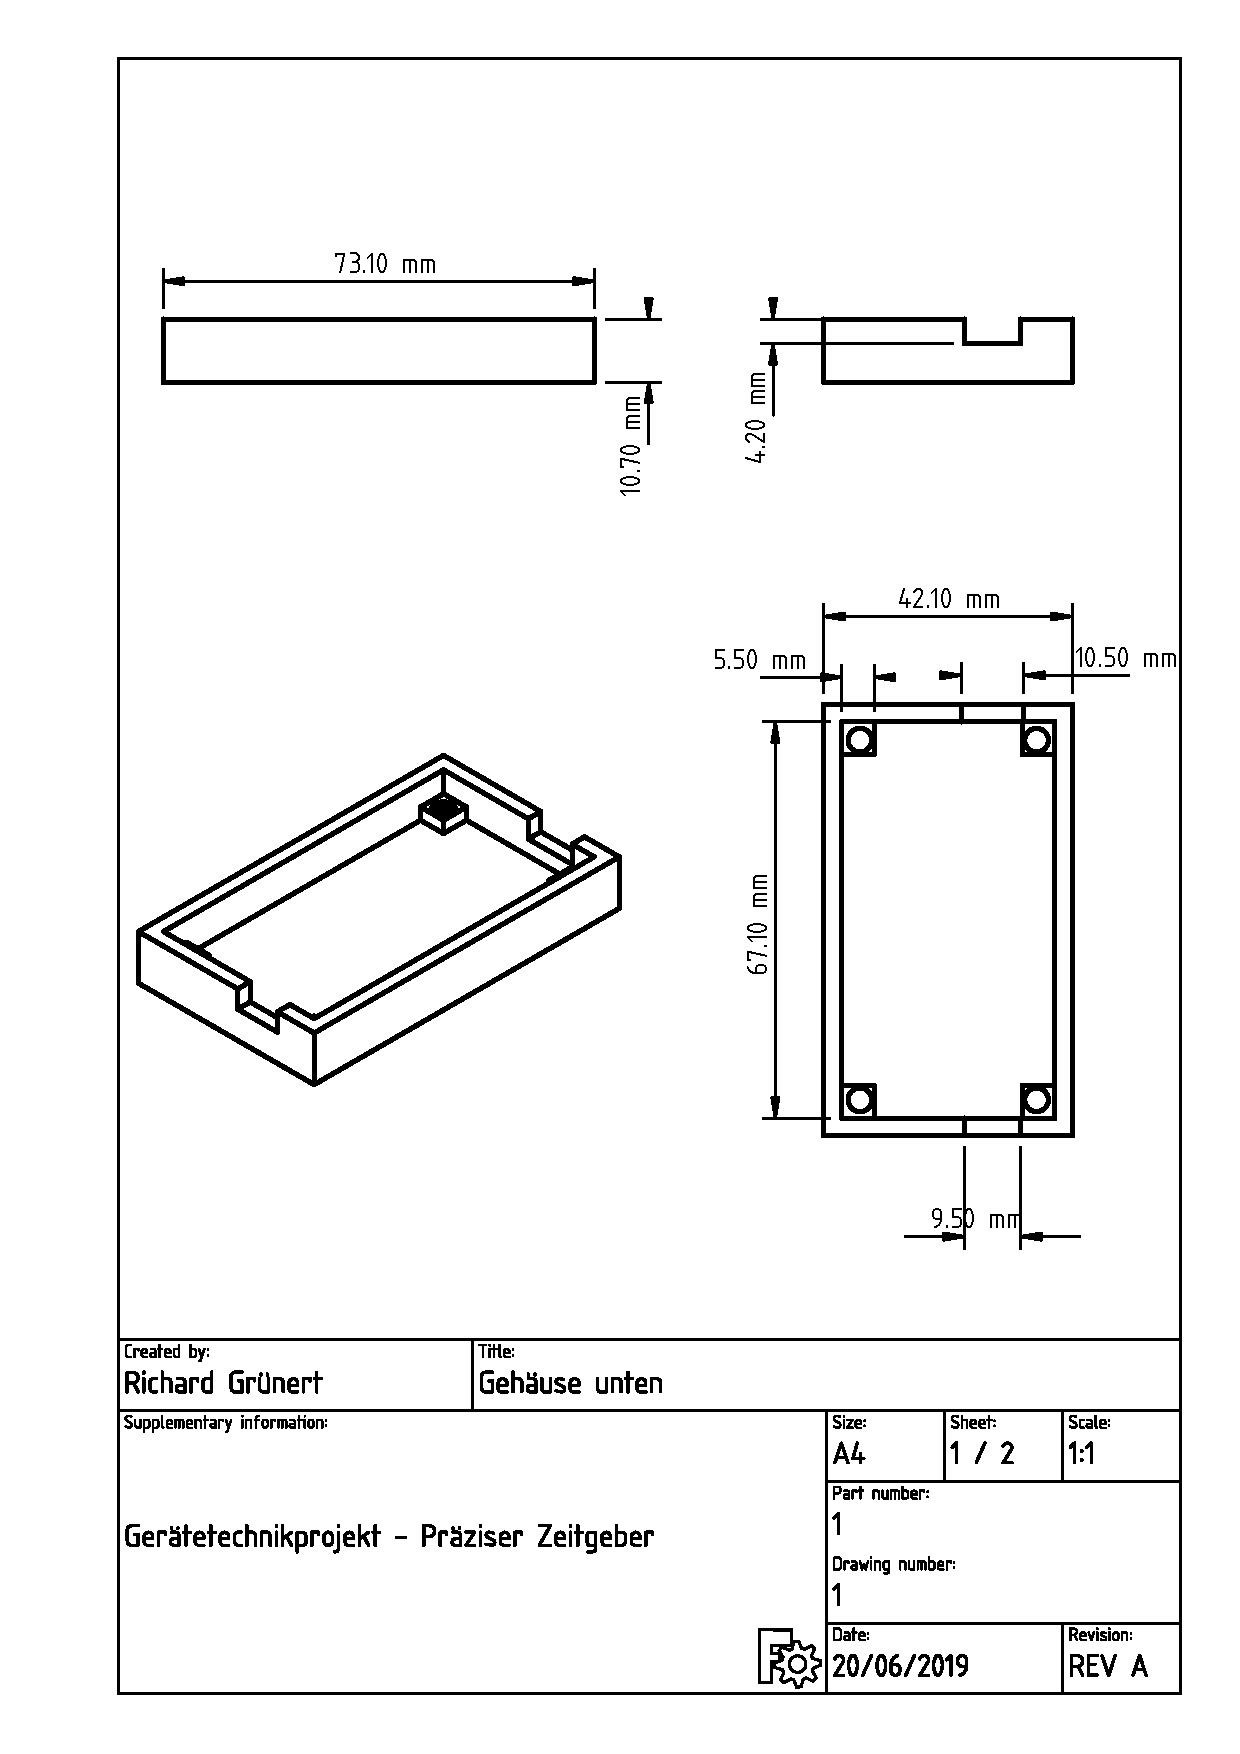
\includepdf{graphics/techdraw_bottom.pdf}
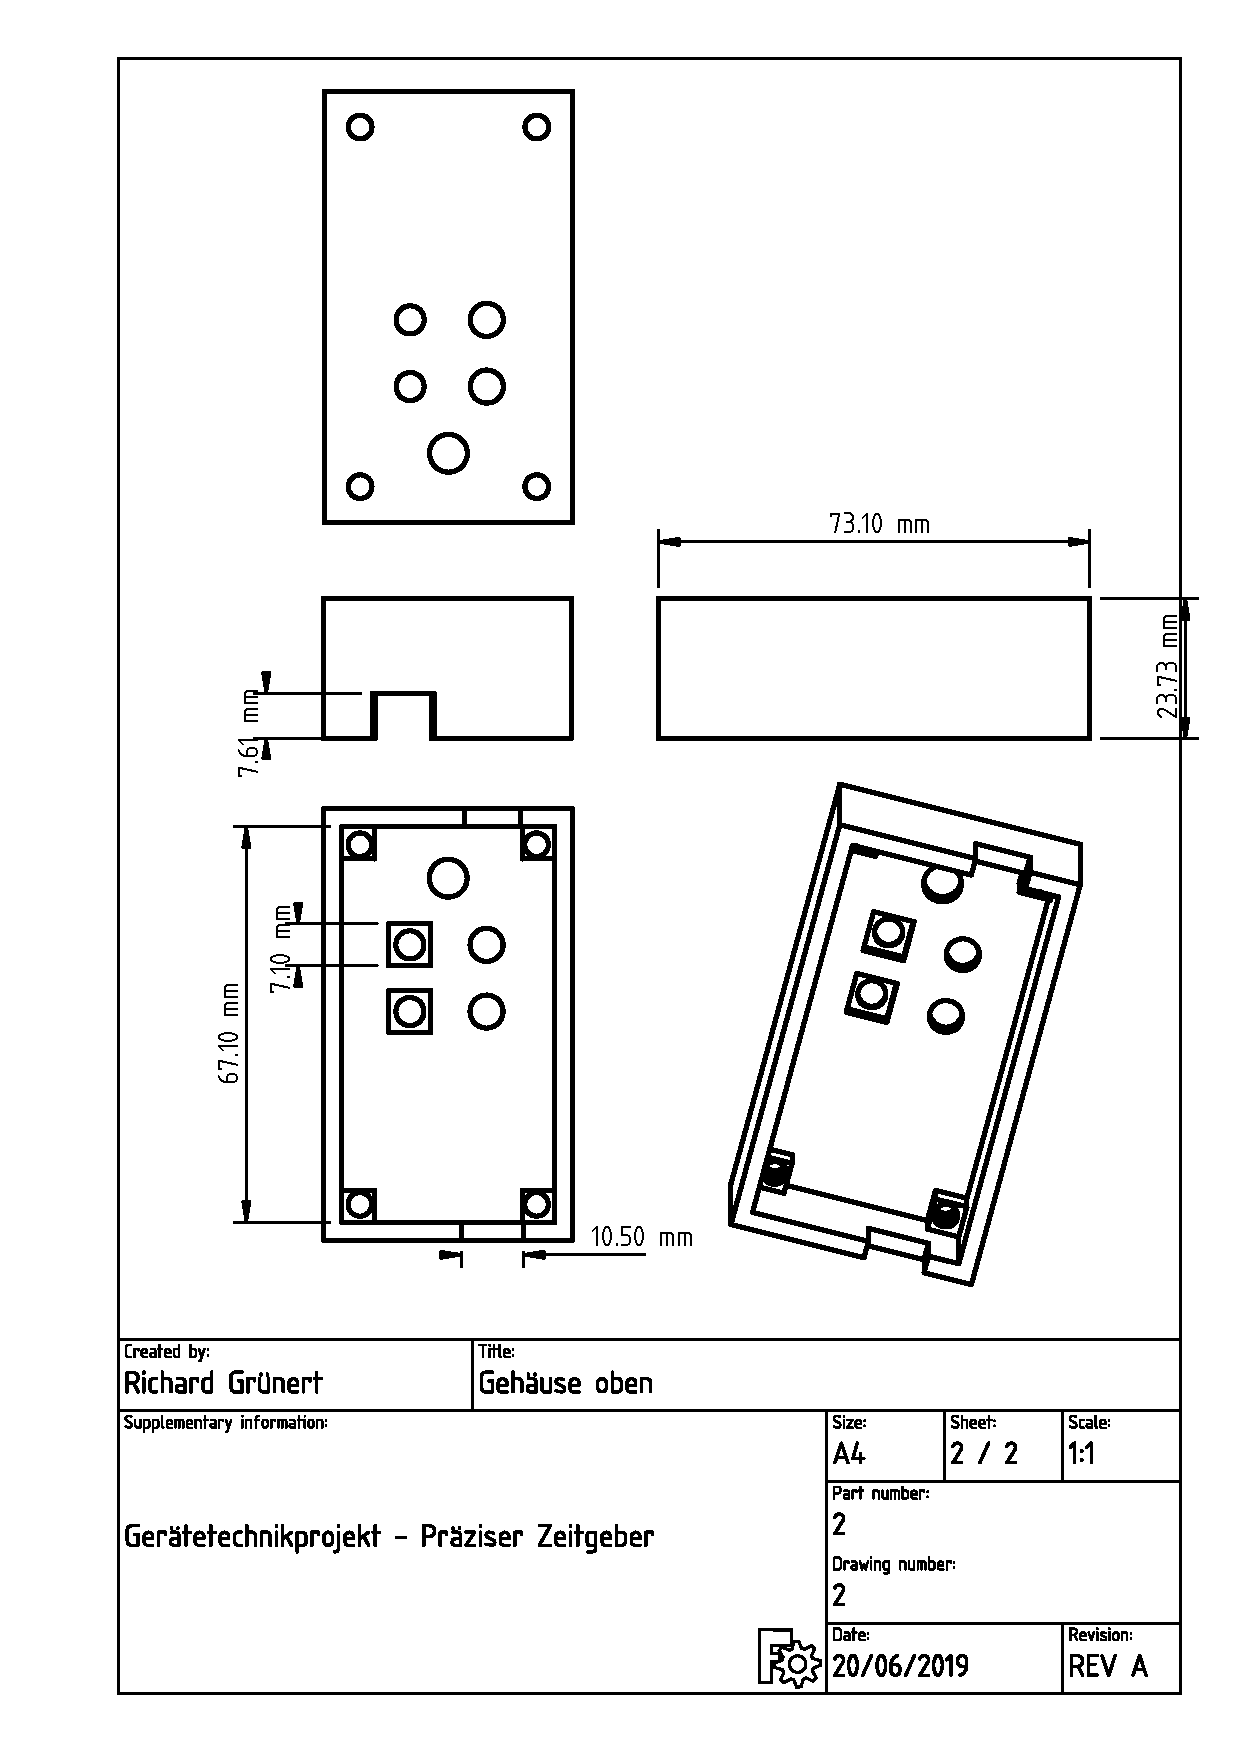
\includepdf{graphics/techdraw_top.pdf}

%\subsection{Datenblätter}
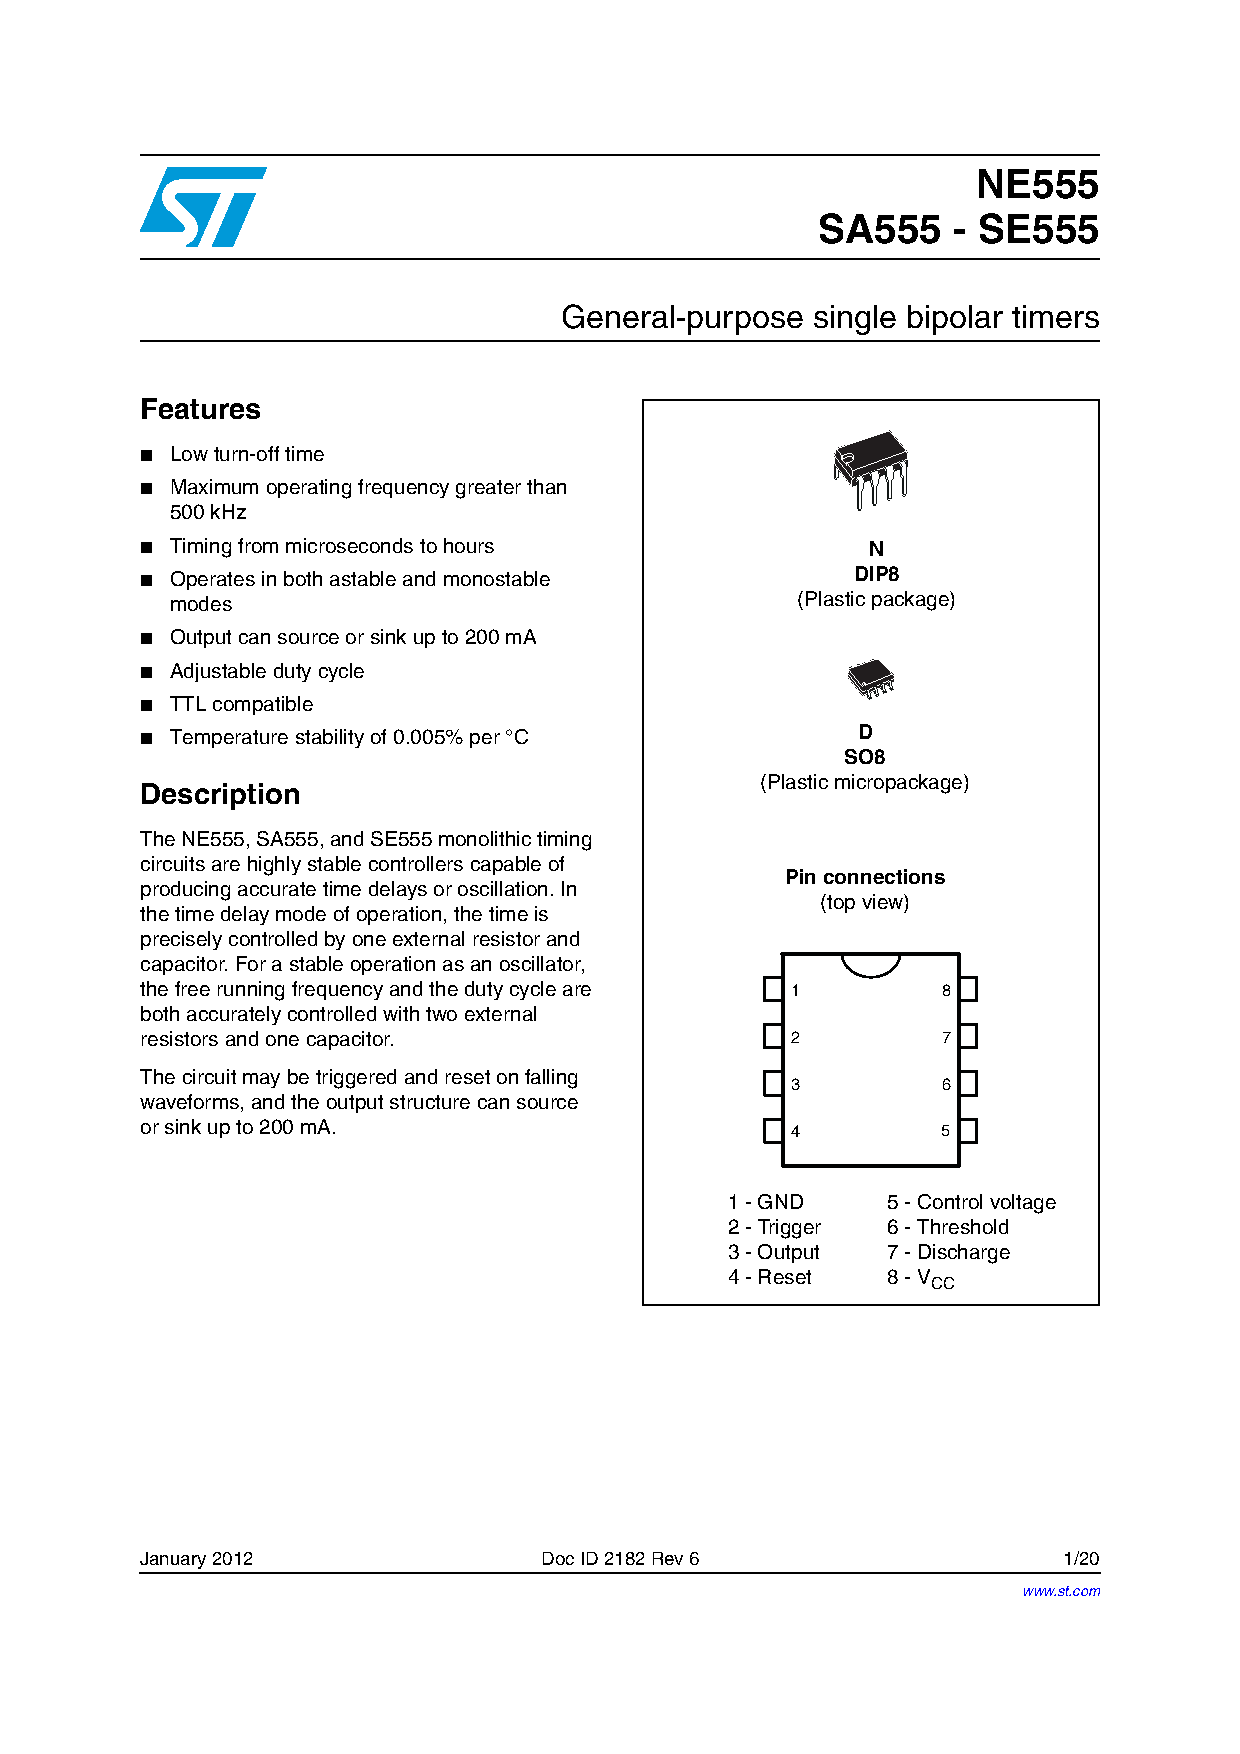
\includepdf[pages={1-5},scale=1,nup=1x3,landscape=true]{555.pdf}
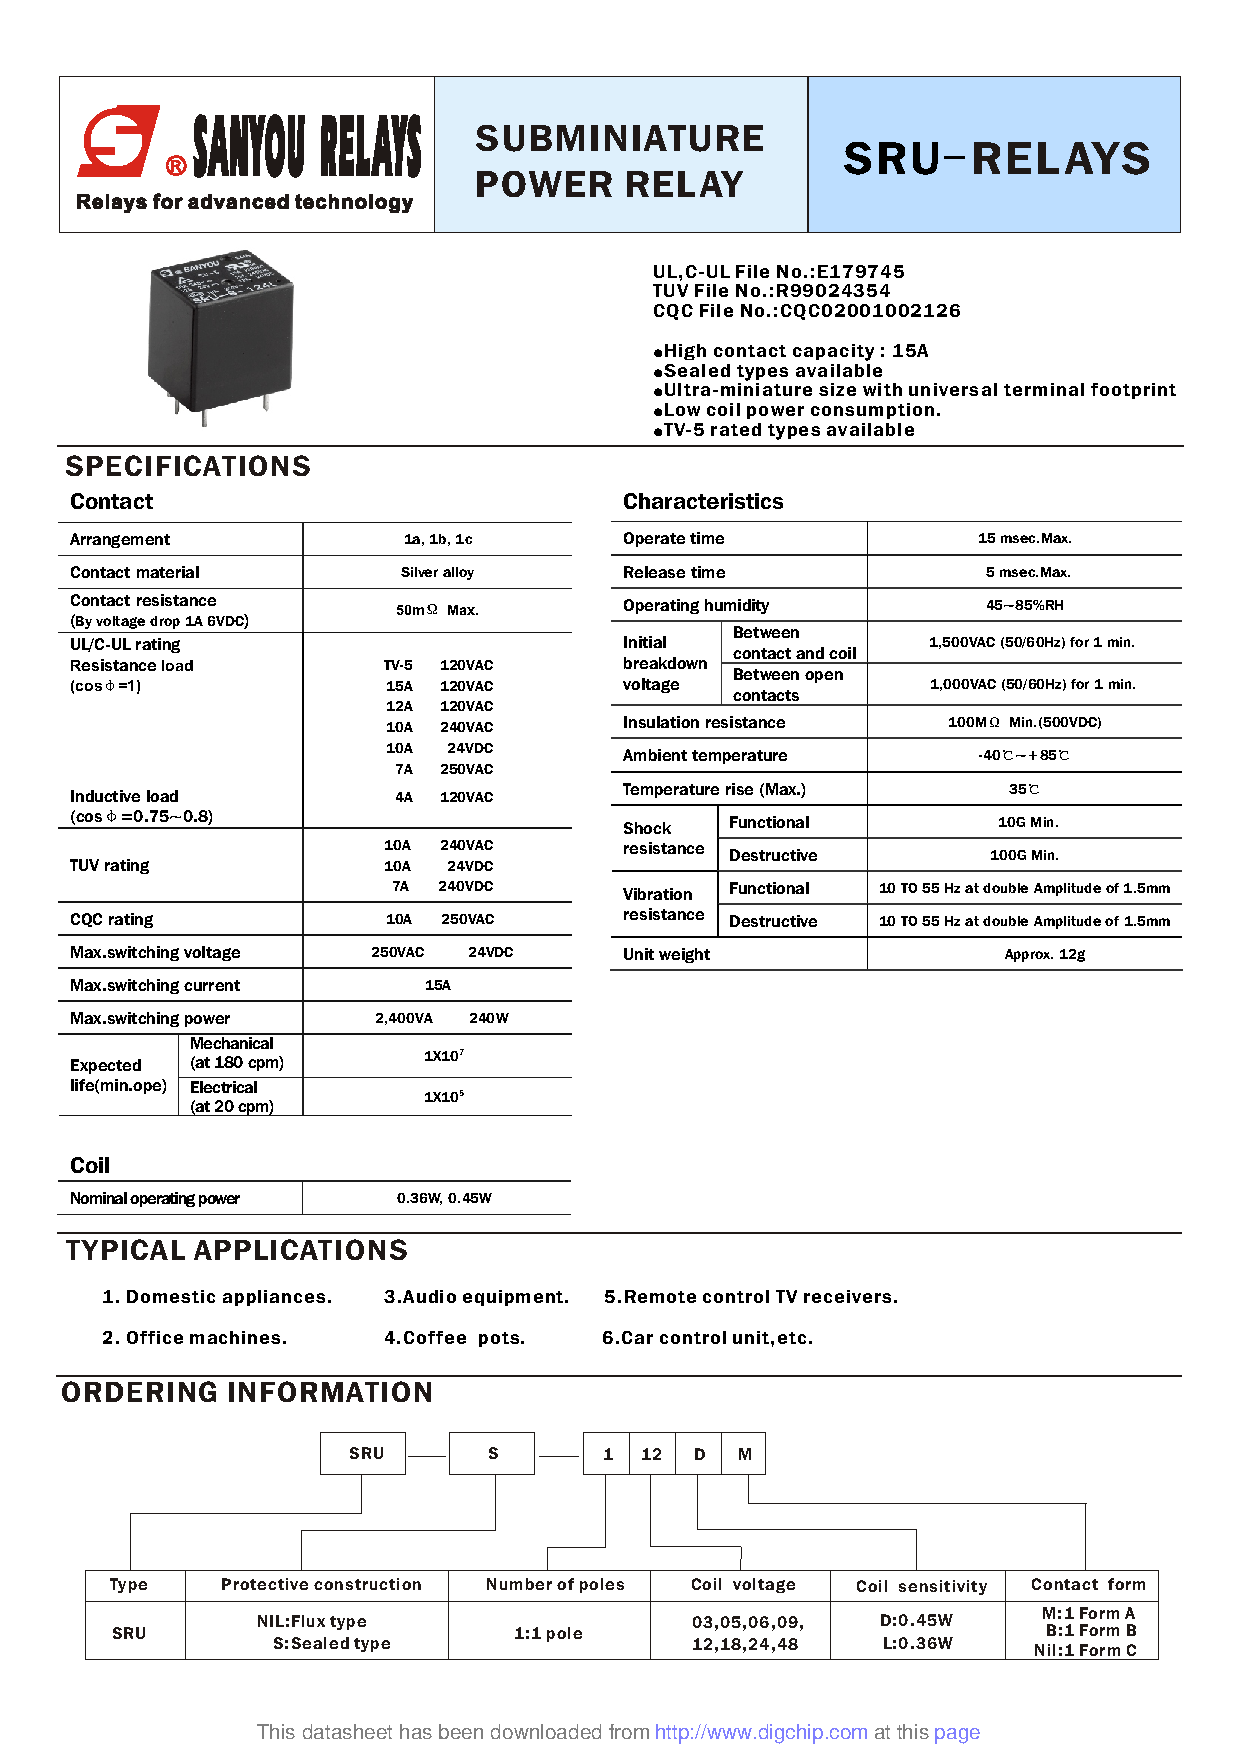
\includepdf[pages={1-},scale=1,nup=1x3,landscape=true]{relais.pdf}
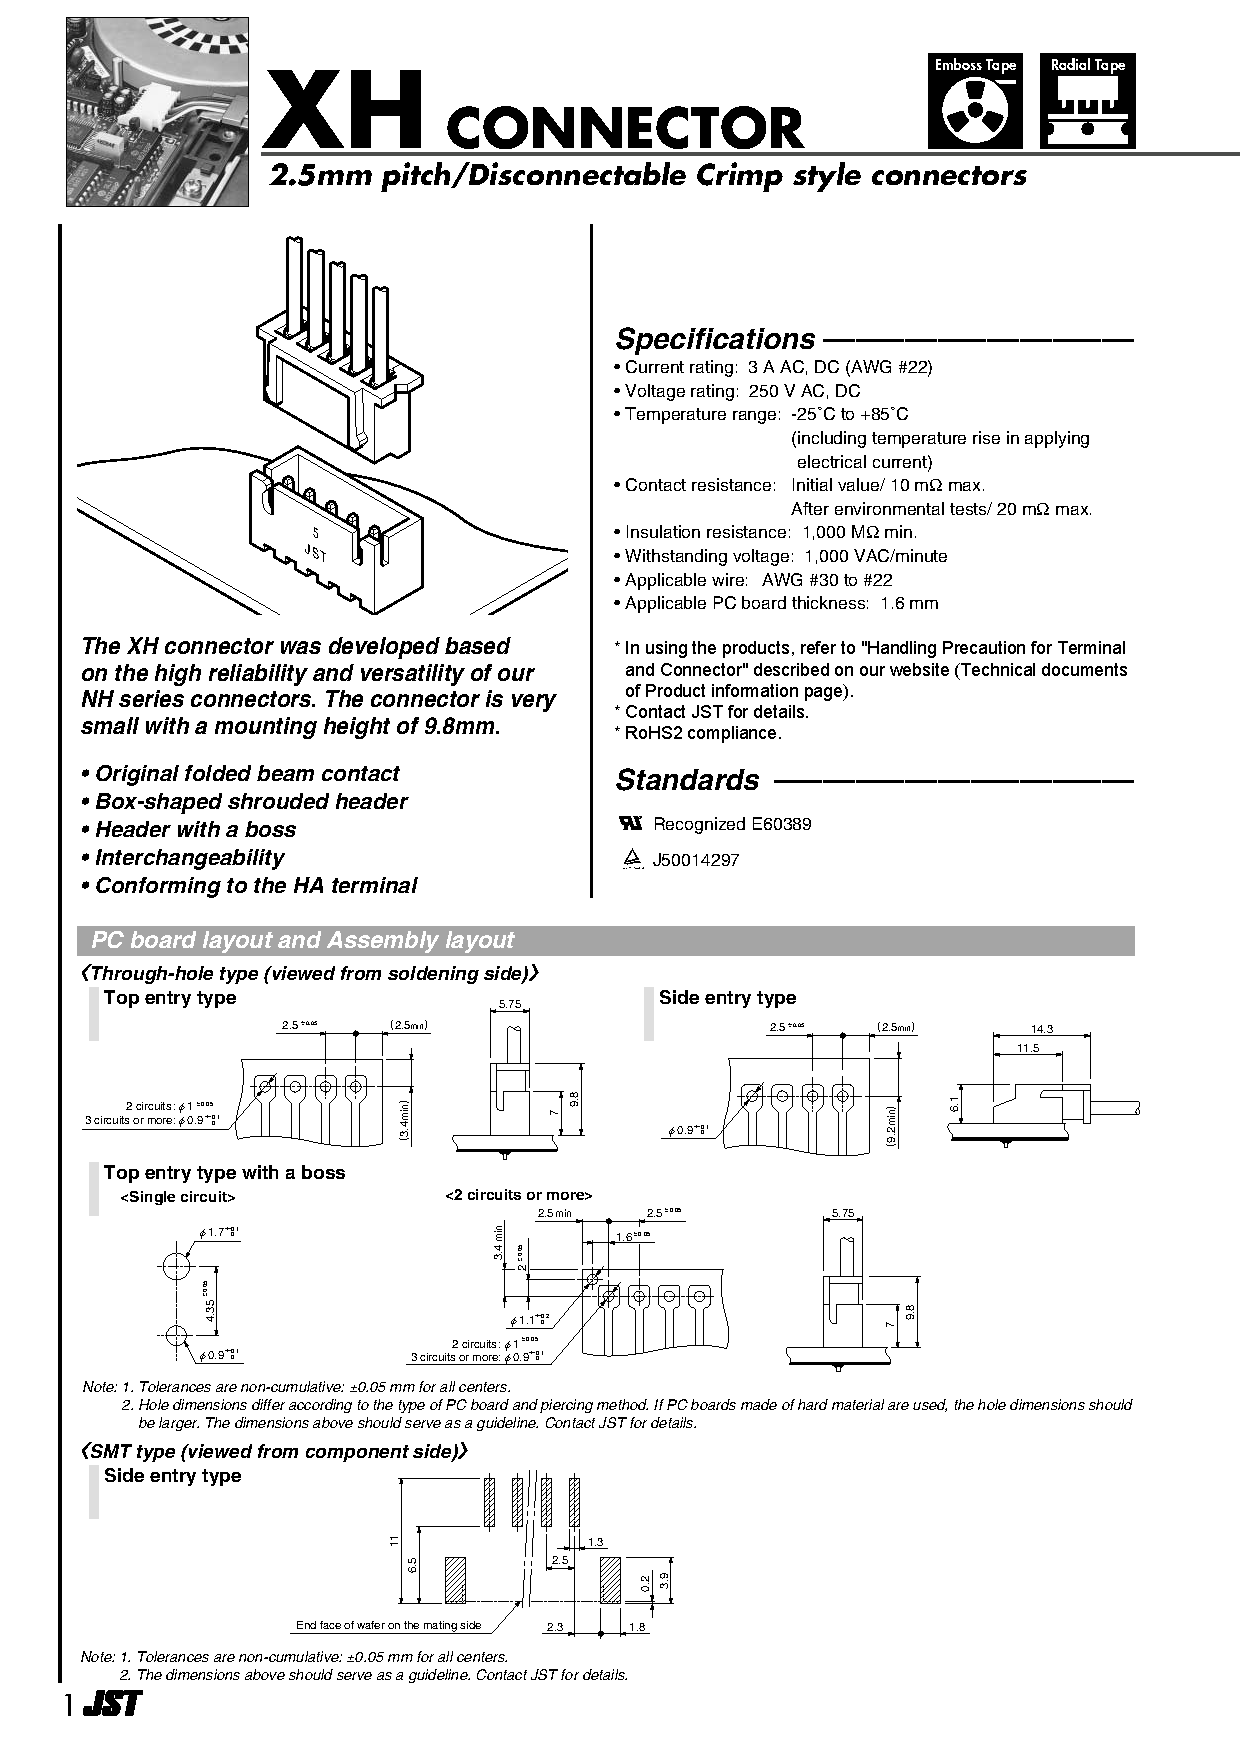
\includepdf[pages={1-4},scale=1,nup=1x3,landscape=true]{jst.pdf}
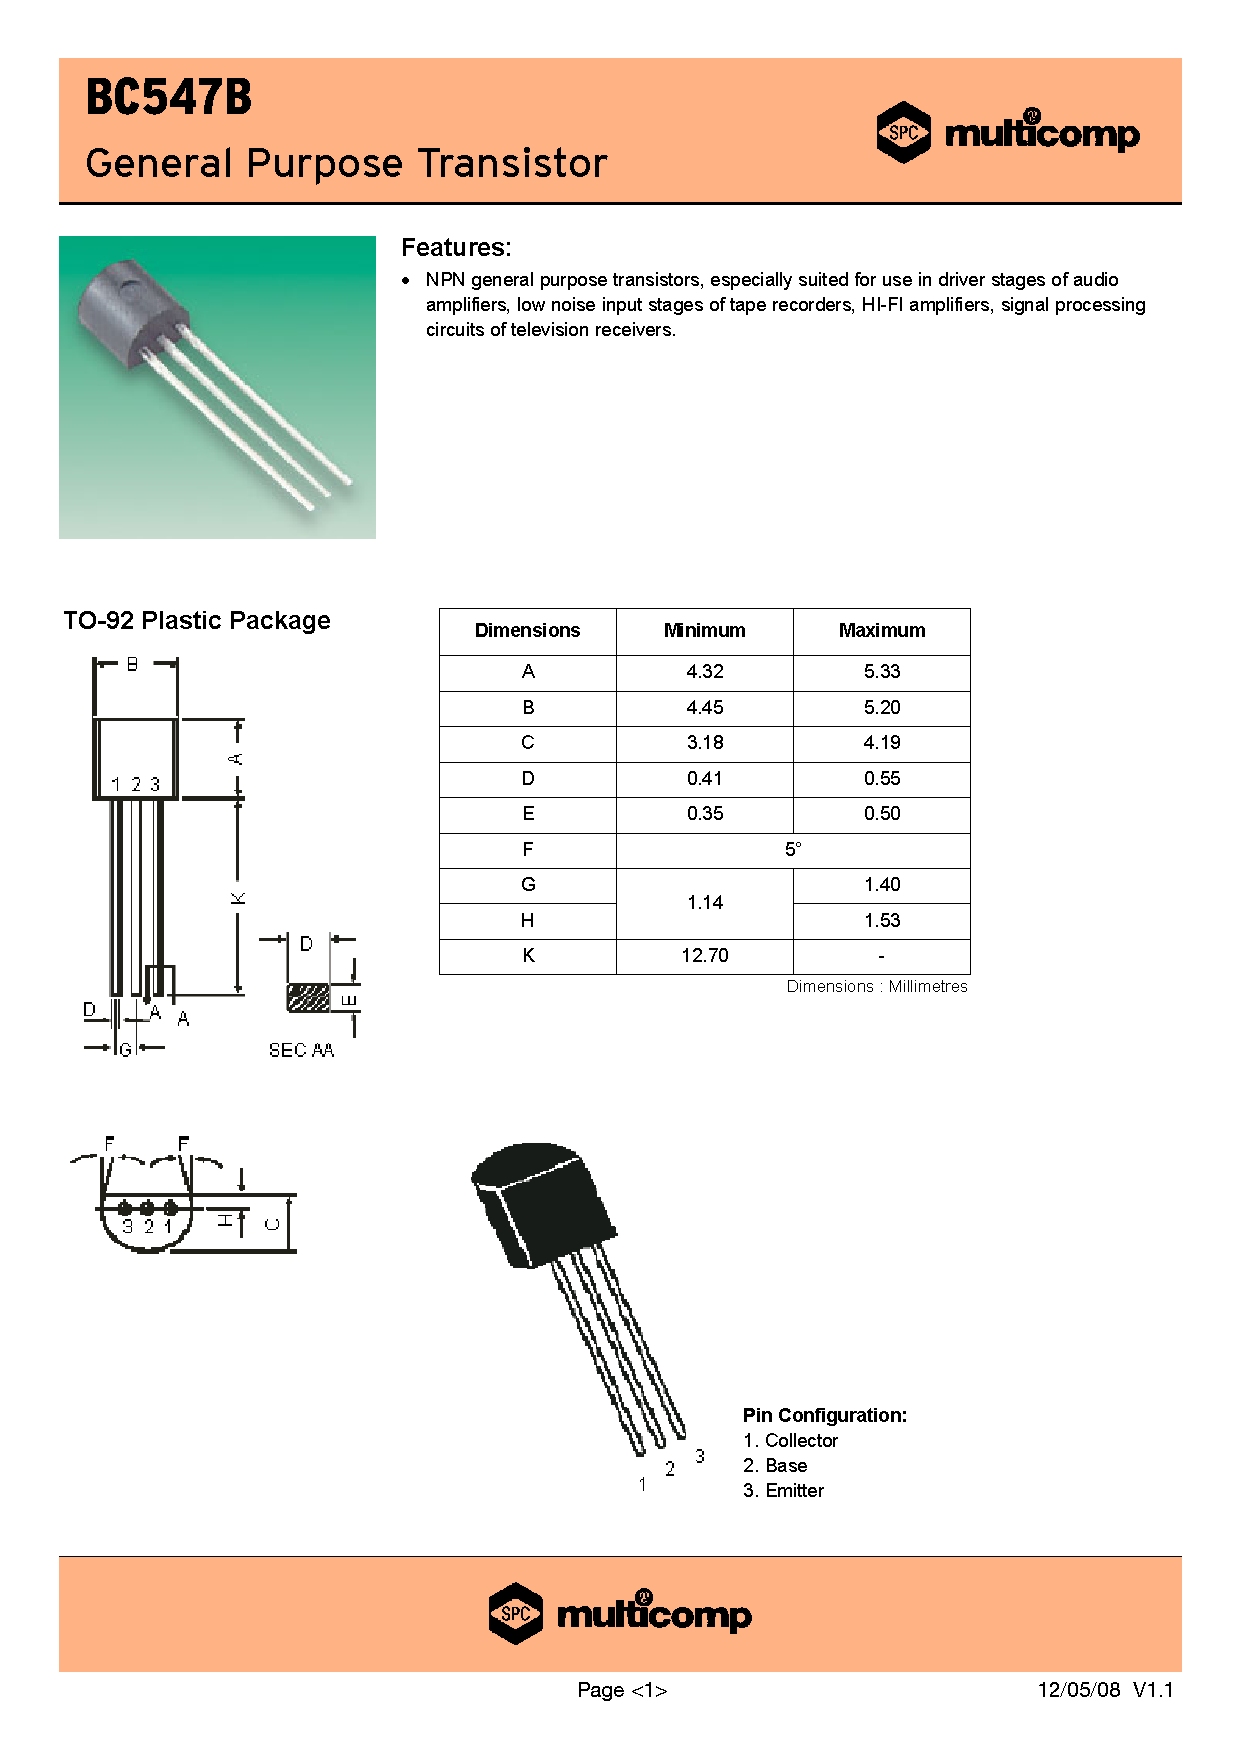
\includepdf[pages={1-3},scale=1,nup=1x3,landscape=true]{transistor.pdf}
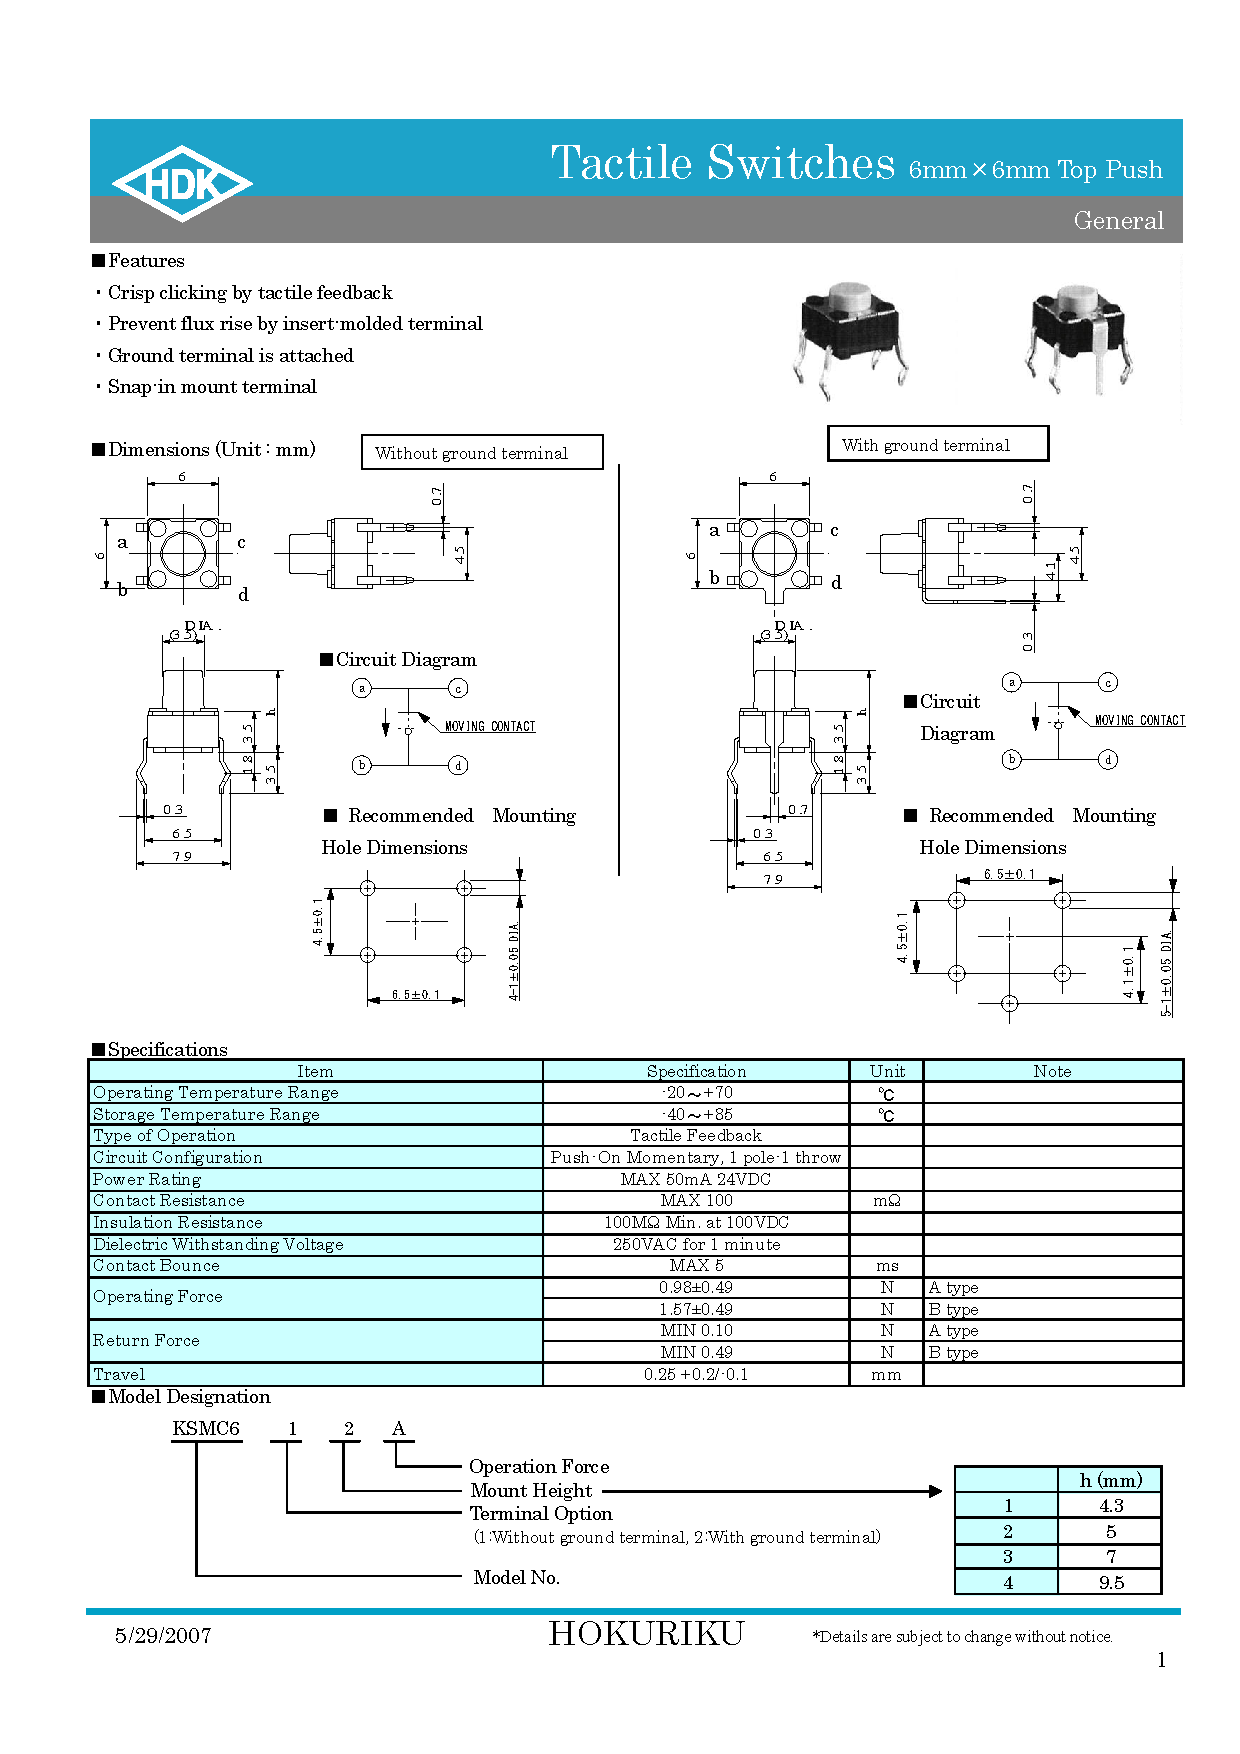
\includepdf[pages={1-},scale=1,nup=1,landscape=false]{schalter.pdf}


\includepdf{eigenstaendigkeit.pdf}

\end{document}
